% Options for packages loaded elsewhere
\PassOptionsToPackage{unicode}{hyperref}
\PassOptionsToPackage{hyphens}{url}
%
\documentclass[
]{book}
\usepackage{amsmath,amssymb}
\usepackage{lmodern}
\usepackage{iftex}
\ifPDFTeX
  \usepackage[T1]{fontenc}
  \usepackage[utf8]{inputenc}
  \usepackage{textcomp} % provide euro and other symbols
\else % if luatex or xetex
  \usepackage{unicode-math}
  \defaultfontfeatures{Scale=MatchLowercase}
  \defaultfontfeatures[\rmfamily]{Ligatures=TeX,Scale=1}
\fi
% Use upquote if available, for straight quotes in verbatim environments
\IfFileExists{upquote.sty}{\usepackage{upquote}}{}
\IfFileExists{microtype.sty}{% use microtype if available
  \usepackage[]{microtype}
  \UseMicrotypeSet[protrusion]{basicmath} % disable protrusion for tt fonts
}{}
\makeatletter
\@ifundefined{KOMAClassName}{% if non-KOMA class
  \IfFileExists{parskip.sty}{%
    \usepackage{parskip}
  }{% else
    \setlength{\parindent}{0pt}
    \setlength{\parskip}{6pt plus 2pt minus 1pt}}
}{% if KOMA class
  \KOMAoptions{parskip=half}}
\makeatother
\usepackage{xcolor}
\usepackage{color}
\usepackage{fancyvrb}
\newcommand{\VerbBar}{|}
\newcommand{\VERB}{\Verb[commandchars=\\\{\}]}
\DefineVerbatimEnvironment{Highlighting}{Verbatim}{commandchars=\\\{\}}
% Add ',fontsize=\small' for more characters per line
\usepackage{framed}
\definecolor{shadecolor}{RGB}{248,248,248}
\newenvironment{Shaded}{\begin{snugshade}}{\end{snugshade}}
\newcommand{\AlertTok}[1]{\textcolor[rgb]{0.94,0.16,0.16}{#1}}
\newcommand{\AnnotationTok}[1]{\textcolor[rgb]{0.56,0.35,0.01}{\textbf{\textit{#1}}}}
\newcommand{\AttributeTok}[1]{\textcolor[rgb]{0.77,0.63,0.00}{#1}}
\newcommand{\BaseNTok}[1]{\textcolor[rgb]{0.00,0.00,0.81}{#1}}
\newcommand{\BuiltInTok}[1]{#1}
\newcommand{\CharTok}[1]{\textcolor[rgb]{0.31,0.60,0.02}{#1}}
\newcommand{\CommentTok}[1]{\textcolor[rgb]{0.56,0.35,0.01}{\textit{#1}}}
\newcommand{\CommentVarTok}[1]{\textcolor[rgb]{0.56,0.35,0.01}{\textbf{\textit{#1}}}}
\newcommand{\ConstantTok}[1]{\textcolor[rgb]{0.00,0.00,0.00}{#1}}
\newcommand{\ControlFlowTok}[1]{\textcolor[rgb]{0.13,0.29,0.53}{\textbf{#1}}}
\newcommand{\DataTypeTok}[1]{\textcolor[rgb]{0.13,0.29,0.53}{#1}}
\newcommand{\DecValTok}[1]{\textcolor[rgb]{0.00,0.00,0.81}{#1}}
\newcommand{\DocumentationTok}[1]{\textcolor[rgb]{0.56,0.35,0.01}{\textbf{\textit{#1}}}}
\newcommand{\ErrorTok}[1]{\textcolor[rgb]{0.64,0.00,0.00}{\textbf{#1}}}
\newcommand{\ExtensionTok}[1]{#1}
\newcommand{\FloatTok}[1]{\textcolor[rgb]{0.00,0.00,0.81}{#1}}
\newcommand{\FunctionTok}[1]{\textcolor[rgb]{0.00,0.00,0.00}{#1}}
\newcommand{\ImportTok}[1]{#1}
\newcommand{\InformationTok}[1]{\textcolor[rgb]{0.56,0.35,0.01}{\textbf{\textit{#1}}}}
\newcommand{\KeywordTok}[1]{\textcolor[rgb]{0.13,0.29,0.53}{\textbf{#1}}}
\newcommand{\NormalTok}[1]{#1}
\newcommand{\OperatorTok}[1]{\textcolor[rgb]{0.81,0.36,0.00}{\textbf{#1}}}
\newcommand{\OtherTok}[1]{\textcolor[rgb]{0.56,0.35,0.01}{#1}}
\newcommand{\PreprocessorTok}[1]{\textcolor[rgb]{0.56,0.35,0.01}{\textit{#1}}}
\newcommand{\RegionMarkerTok}[1]{#1}
\newcommand{\SpecialCharTok}[1]{\textcolor[rgb]{0.00,0.00,0.00}{#1}}
\newcommand{\SpecialStringTok}[1]{\textcolor[rgb]{0.31,0.60,0.02}{#1}}
\newcommand{\StringTok}[1]{\textcolor[rgb]{0.31,0.60,0.02}{#1}}
\newcommand{\VariableTok}[1]{\textcolor[rgb]{0.00,0.00,0.00}{#1}}
\newcommand{\VerbatimStringTok}[1]{\textcolor[rgb]{0.31,0.60,0.02}{#1}}
\newcommand{\WarningTok}[1]{\textcolor[rgb]{0.56,0.35,0.01}{\textbf{\textit{#1}}}}
\usepackage{longtable,booktabs,array}
\usepackage{calc} % for calculating minipage widths
% Correct order of tables after \paragraph or \subparagraph
\usepackage{etoolbox}
\makeatletter
\patchcmd\longtable{\par}{\if@noskipsec\mbox{}\fi\par}{}{}
\makeatother
% Allow footnotes in longtable head/foot
\IfFileExists{footnotehyper.sty}{\usepackage{footnotehyper}}{\usepackage{footnote}}
\makesavenoteenv{longtable}
\usepackage{graphicx}
\makeatletter
\def\maxwidth{\ifdim\Gin@nat@width>\linewidth\linewidth\else\Gin@nat@width\fi}
\def\maxheight{\ifdim\Gin@nat@height>\textheight\textheight\else\Gin@nat@height\fi}
\makeatother
% Scale images if necessary, so that they will not overflow the page
% margins by default, and it is still possible to overwrite the defaults
% using explicit options in \includegraphics[width, height, ...]{}
\setkeys{Gin}{width=\maxwidth,height=\maxheight,keepaspectratio}
% Set default figure placement to htbp
\makeatletter
\def\fps@figure{htbp}
\makeatother
\setlength{\emergencystretch}{3em} % prevent overfull lines
\providecommand{\tightlist}{%
  \setlength{\itemsep}{0pt}\setlength{\parskip}{0pt}}
\setcounter{secnumdepth}{5}
\usepackage{booktabs}
\ifLuaTeX
  \usepackage{selnolig}  % disable illegal ligatures
\fi
\usepackage[]{natbib}
\bibliographystyle{plainnat}
\IfFileExists{bookmark.sty}{\usepackage{bookmark}}{\usepackage{hyperref}}
\IfFileExists{xurl.sty}{\usepackage{xurl}}{} % add URL line breaks if available
\urlstyle{same} % disable monospaced font for URLs
\hypersetup{
  pdftitle={Biology 3315 Molecular Evolution and Phylogenetics},
  pdfauthor={Dr.~Ido Hatam},
  hidelinks,
  pdfcreator={LaTeX via pandoc}}

\title{Biology 3315 Molecular Evolution and Phylogenetics}
\usepackage{etoolbox}
\makeatletter
\providecommand{\subtitle}[1]{% add subtitle to \maketitle
  \apptocmd{\@title}{\par {\large #1 \par}}{}{}
}
\makeatother
\subtitle{Lab manual}
\author{Dr.~Ido Hatam}
\date{February 13, 2023}

\usepackage{amsthm}
\newtheorem{theorem}{Theorem}[chapter]
\newtheorem{lemma}{Lemma}[chapter]
\newtheorem{corollary}{Corollary}[chapter]
\newtheorem{proposition}{Proposition}[chapter]
\newtheorem{conjecture}{Conjecture}[chapter]
\theoremstyle{definition}
\newtheorem{definition}{Definition}[chapter]
\theoremstyle{definition}
\newtheorem{example}{Example}[chapter]
\theoremstyle{definition}
\newtheorem{exercise}{Exercise}[chapter]
\theoremstyle{definition}
\newtheorem{hypothesis}{Hypothesis}[chapter]
\theoremstyle{remark}
\newtheorem*{remark}{Remark}
\newtheorem*{solution}{Solution}
\begin{document}
\maketitle

{
\setcounter{tocdepth}{1}
\tableofcontents
}
\hypertarget{an-introduction-to-the-lab}{%
\chapter*{\texorpdfstring{\textbf{An introduction to the lab}}{An introduction to the lab}}\label{an-introduction-to-the-lab}}
\addcontentsline{toc}{chapter}{\textbf{An introduction to the lab}}

This is a \emph{sample} book written in \textbf{Markdown}. You can use anything that Pandoc's Markdown supports; for example, a math equation \(a^2 + b^2 = c^2\).

\hypertarget{how-to-get-the-most-out-of-the-lab}{%
\section*{\texorpdfstring{\textbf{How to get the most out of the lab}}{How to get the most out of the lab}}\label{how-to-get-the-most-out-of-the-lab}}
\addcontentsline{toc}{section}{\textbf{How to get the most out of the lab}}

Each \textbf{bookdown} chapter is an .Rmd file, and each .Rmd file can contain one (and only one) chapter. A chapter \emph{must} start with a first-level heading: \texttt{\#\ A\ good\ chapter}, and can contain one (and only one) first-level heading.

Use second-level and higher headings within chapters like: \texttt{\#\#\ A\ short\ section} or \texttt{\#\#\#\ An\ even\ shorter\ section}.

The \texttt{index.Rmd} file is required, and is also your first book chapter. It will be the homepage when you render the book.

\hypertarget{render-book}{%
\section{Render book}\label{render-book}}

You can render the HTML version of this example book without changing anything:

\begin{enumerate}
\def\labelenumi{\arabic{enumi}.}
\item
  Find the \textbf{Build} pane in the RStudio IDE, and
\item
  Click on \textbf{Build Book}, then select your output format, or select ``All formats'' if you'd like to use multiple formats from the same book source files.
\end{enumerate}

Or build the book from the R console:

\begin{Shaded}
\begin{Highlighting}[]
\NormalTok{bookdown}\SpecialCharTok{::}\FunctionTok{render\_book}\NormalTok{()}
\end{Highlighting}
\end{Shaded}

To render this example to PDF as a \texttt{bookdown::pdf\_book}, you'll need to install XeLaTeX. You are recommended to install TinyTeX (which includes XeLaTeX): \url{https://yihui.org/tinytex/}.

\hypertarget{preview-book}{%
\section{Preview book}\label{preview-book}}

As you work, you may start a local server to live preview this HTML book. This preview will update as you edit the book when you save individual .Rmd files. You can start the server in a work session by using the RStudio add-in ``Preview book'', or from the R console:

\begin{Shaded}
\begin{Highlighting}[]
\NormalTok{bookdown}\SpecialCharTok{::}\FunctionTok{serve\_book}\NormalTok{()}
\end{Highlighting}
\end{Shaded}

\hypertarget{lab-1-introduction-to-the-r-programming-language-and-the-r-studio-ide}{%
\chapter*{\texorpdfstring{\textbf{Lab 1 introduction to the R programming language and the R studio IDE}}{Lab 1 introduction to the R programming language and the R studio IDE}}\label{lab-1-introduction-to-the-r-programming-language-and-the-r-studio-ide}}
\addcontentsline{toc}{chapter}{\textbf{Lab 1 introduction to the R programming language and the R studio IDE}}

\hypertarget{learning-objectives}{%
\section*{\texorpdfstring{\textbf{Learning objectives}}{Learning objectives}}\label{learning-objectives}}
\addcontentsline{toc}{section}{\textbf{Learning objectives}}

Click to expand

\textbf{By the end of this lab you will be able to:}

\begin{itemize}
\item
  Install the R interpreter and the Rstudio integrated development environment
\item
  Demonstrate the ability to install and load packages from a variety of repositories including development versions from github
\item
  Understand the different components of the Rstudio environment
\item
  Demonstrate mastery of R object and data types including indexing, subseting and manipulating objects
\item
  Demonstrate the ability to call and chain functions
\end{itemize}

\hypertarget{getting-started}{%
\section*{\texorpdfstring{\textbf{Getting started}}{Getting started}}\label{getting-started}}
\addcontentsline{toc}{section}{\textbf{Getting started}}

\hypertarget{what-is-r}{%
\subsection*{\texorpdfstring{\textbf{What is R?}}{What is R?}}\label{what-is-r}}
\addcontentsline{toc}{subsection}{\textbf{What is R?}}

R is a free and open source programming language, operating as a \href{http://www.gnu.org/}{GUN project}. The R language is maintained and supported by the \href{https://www.r-project.org/foundation/}{R Foundation for Statistical Computing}.

\begin{quote}
``R is a functional programming language and environment for statistical computing and graphics''

--- The R dev team
\end{quote}

R is best known as a programming language with strong capabilities of
manipulation, exploration and statistical analysis of data from diverse
types and sources. However, it also provides an environment for data
handling, graphical representation of data as well as data reporting.
R is a great platform for documentation and in fact this entire lab
manual was written in R using the rmarkdown package.

\hypertarget{why-use-r}{%
\subsection*{\texorpdfstring{\textbf{Why use R?}}{Why use R?}}\label{why-use-r}}
\addcontentsline{toc}{subsection}{\textbf{Why use R?}}

\begin{itemize}
\tightlist
\item
  Open source and free

  \begin{itemize}
  \tightlist
  \item
    Available on all major platform
  \end{itemize}
\item
  Large community of users and developers (over 2M users in academia, government, and industry)
\item
  Thousands of open source packages aimed at the analysis of biological data in general and genomic and evolutionary data in particular
\item
  Customizable and allows for the construction of pipelines
\item
  Reproducible analysis
\end{itemize}

\hypertarget{downloading-and-installing-r-and-rstudio-desktop}{%
\subsection*{\texorpdfstring{\textbf{Downloading and installing R and RStudio desktop}}{Downloading and installing R and RStudio desktop}}\label{downloading-and-installing-r-and-rstudio-desktop}}
\addcontentsline{toc}{subsection}{\textbf{Downloading and installing R and RStudio desktop}}

To download R, go to the \href{https://cran.r-project.org/mirrors.html}{R download page} select the SFU mirror then select your operating system and download and install both 32 and 64 bit versions.

To download RStudio desktop, go to the \href{https://posit.co/download/rstudio-desktop/}{RStudio download page} and download the free RStudio desktop version.

\begin{center}\rule{0.5\linewidth}{0.5pt}\end{center}

\begin{quote}
Note that you must download and install both R and RStudio in order to be able to work with R in the RStudio IDE.
Note that it is important that you have the most uptodate verssion of R, even if R is already installed on your computer
make sure to update it. If using Windows you can use the \href{https://github.com/talgalili/installr}{installr package} to
update R.
\end{quote}

\begin{center}\rule{0.5\linewidth}{0.5pt}\end{center}

\hypertarget{the-r-interpreter}{%
\subsection*{\texorpdfstring{\textbf{The R interpreter}}{The R interpreter}}\label{the-r-interpreter}}
\addcontentsline{toc}{subsection}{\textbf{The R interpreter}}

Generally speaking, R is an interpreted language, and it's human readable code cannot be directly converted to machine code
by the operating system. Therefore, it needs an interpreter to translate the human readable code to a format understood by
the operating system and the processing unit as the code runs.

\begin{figure}

{\centering 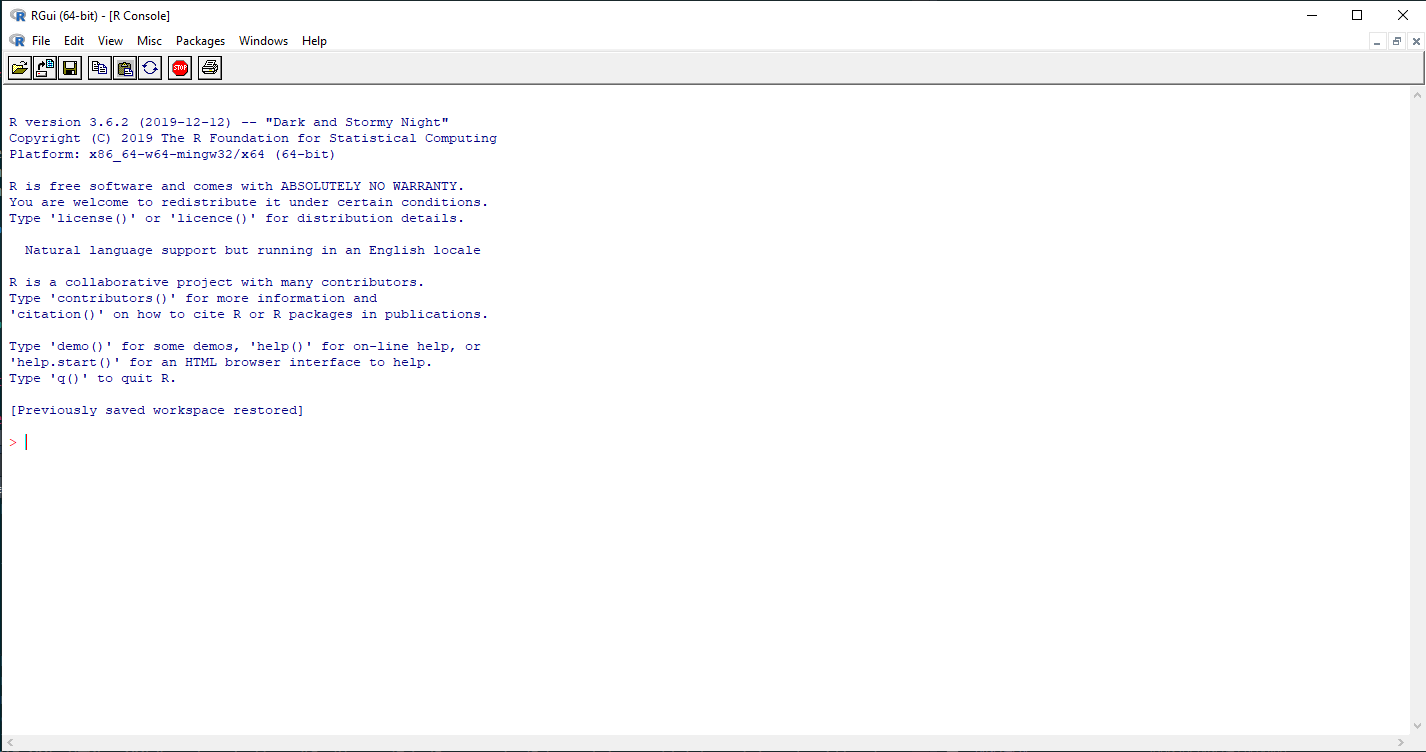
\includegraphics[width=1\linewidth]{figs/Rcons} 

}

\caption{The R console}\label{fig:unnamed-chunk-4}
\end{figure}

The R console is an R interpreter with a very simple GUI. It allows you to write and run your code line by line just like you would in a terminal.

Console input and output:

\begin{Shaded}
\begin{Highlighting}[]
\DecValTok{1}\SpecialCharTok{+}\DecValTok{1}
\end{Highlighting}
\end{Shaded}

\begin{verbatim}
## [1] 2
\end{verbatim}

\begin{Shaded}
\begin{Highlighting}[]
\DecValTok{3}\SpecialCharTok{*}\DecValTok{3}
\end{Highlighting}
\end{Shaded}

\begin{verbatim}
## [1] 9
\end{verbatim}

\begin{Shaded}
\begin{Highlighting}[]
\DecValTok{4}\SpecialCharTok{/}\DecValTok{2}
\end{Highlighting}
\end{Shaded}

\begin{verbatim}
## [1] 2
\end{verbatim}

\begin{Shaded}
\begin{Highlighting}[]
\DecValTok{4}\SpecialCharTok{\^{}}\DecValTok{2}
\end{Highlighting}
\end{Shaded}

\begin{verbatim}
## [1] 16
\end{verbatim}

\begin{Shaded}
\begin{Highlighting}[]
\FunctionTok{print}\NormalTok{(}\StringTok{"Hello world"}\NormalTok{)}
\end{Highlighting}
\end{Shaded}

\begin{verbatim}
## [1] "Hello world"
\end{verbatim}

In the example code above\ldots{} something about the console interpreting white and in gray output\ldots{} Furthermore, the print function was called to print the famous ``Hello world'' combo no coding workshop is complete without.

\hypertarget{short-console-exercise}{%
\subsubsection*{\texorpdfstring{\textbf{Short console exercise}}{Short console exercise}}\label{short-console-exercise}}
\addcontentsline{toc}{subsubsection}{\textbf{Short console exercise}}

Now let's get you to work. The following lines of code will assign values to the variables ``j'',``k'', and ``rowling'' (we will
discuss variable assignment in R later in this lab).
Open the R console on your computer and run them.

\begin{Shaded}
\begin{Highlighting}[]
\NormalTok{j }\OtherTok{\textless{}{-}} \StringTok{"Harry"}
\NormalTok{k }\OtherTok{\textless{}{-}} \StringTok{"Poter"}
\NormalTok{rowling }\OtherTok{\textless{}{-}} \FunctionTok{data.frame}\NormalTok{(}\AttributeTok{First\_name =}\NormalTok{ j,}\AttributeTok{Last\_name =}\NormalTok{ k)}
\end{Highlighting}
\end{Shaded}

Notice that no output was generated, since you only assigned values to some variables. You can get the interpreter to
output the value of each variable by calling them in the console. Try it for each of them.
As you can see, the variables are stored in memory. This is evident by the output generated when you called the
variables in the console. Furthermore, without knowing too much R, you probably already guessed that not all
variables are created equal and that there is some differences between rowling and the rest of the variables.
However, the console doesn't let one see immediately how many variables one stored in memory, nor does it let one see
their names, memory allocation, type, etc. In order to see those using just the console you would have to call an
array of functions.
For example try running the following function is your console.

\begin{Shaded}
\begin{Highlighting}[]
\FunctionTok{ls}\NormalTok{()}
\end{Highlighting}
\end{Shaded}

\begin{center}\rule{0.5\linewidth}{0.5pt}\end{center}

\begin{quote}
If you are familiar with UNIX based operating systems, you probably recognized that ls is short for list.
When running the ls() function in the console, the the output will list all stored variables. But as you may
notice, this is about all it does. You can also imagine that this is not the most efficient way to keep track of the
variables you declare when working with more than a couple variables (which is sometimes required). In order to keep
things streamlined and organized, it is advisable to work with an Integrated Development Environment (IDE), which
allows you to have better control of code editing, variable storage, console output etc. R has several IDEs, however
the most popular by far is RStudio.
\end{quote}

\begin{center}\rule{0.5\linewidth}{0.5pt}\end{center}

\hypertarget{the-rstudio-ide}{%
\subsection*{\texorpdfstring{\textbf{The RStudio IDE}}{The RStudio IDE}}\label{the-rstudio-ide}}
\addcontentsline{toc}{subsection}{\textbf{The RStudio IDE}}

As mentioned above, RStudio is an integrated development environment (IDE) for R. It is highly customizable but its
default setting include four panes, a text editor pane, a console pane, a global environment pane, and an output
pane.

\begin{figure}

{\centering 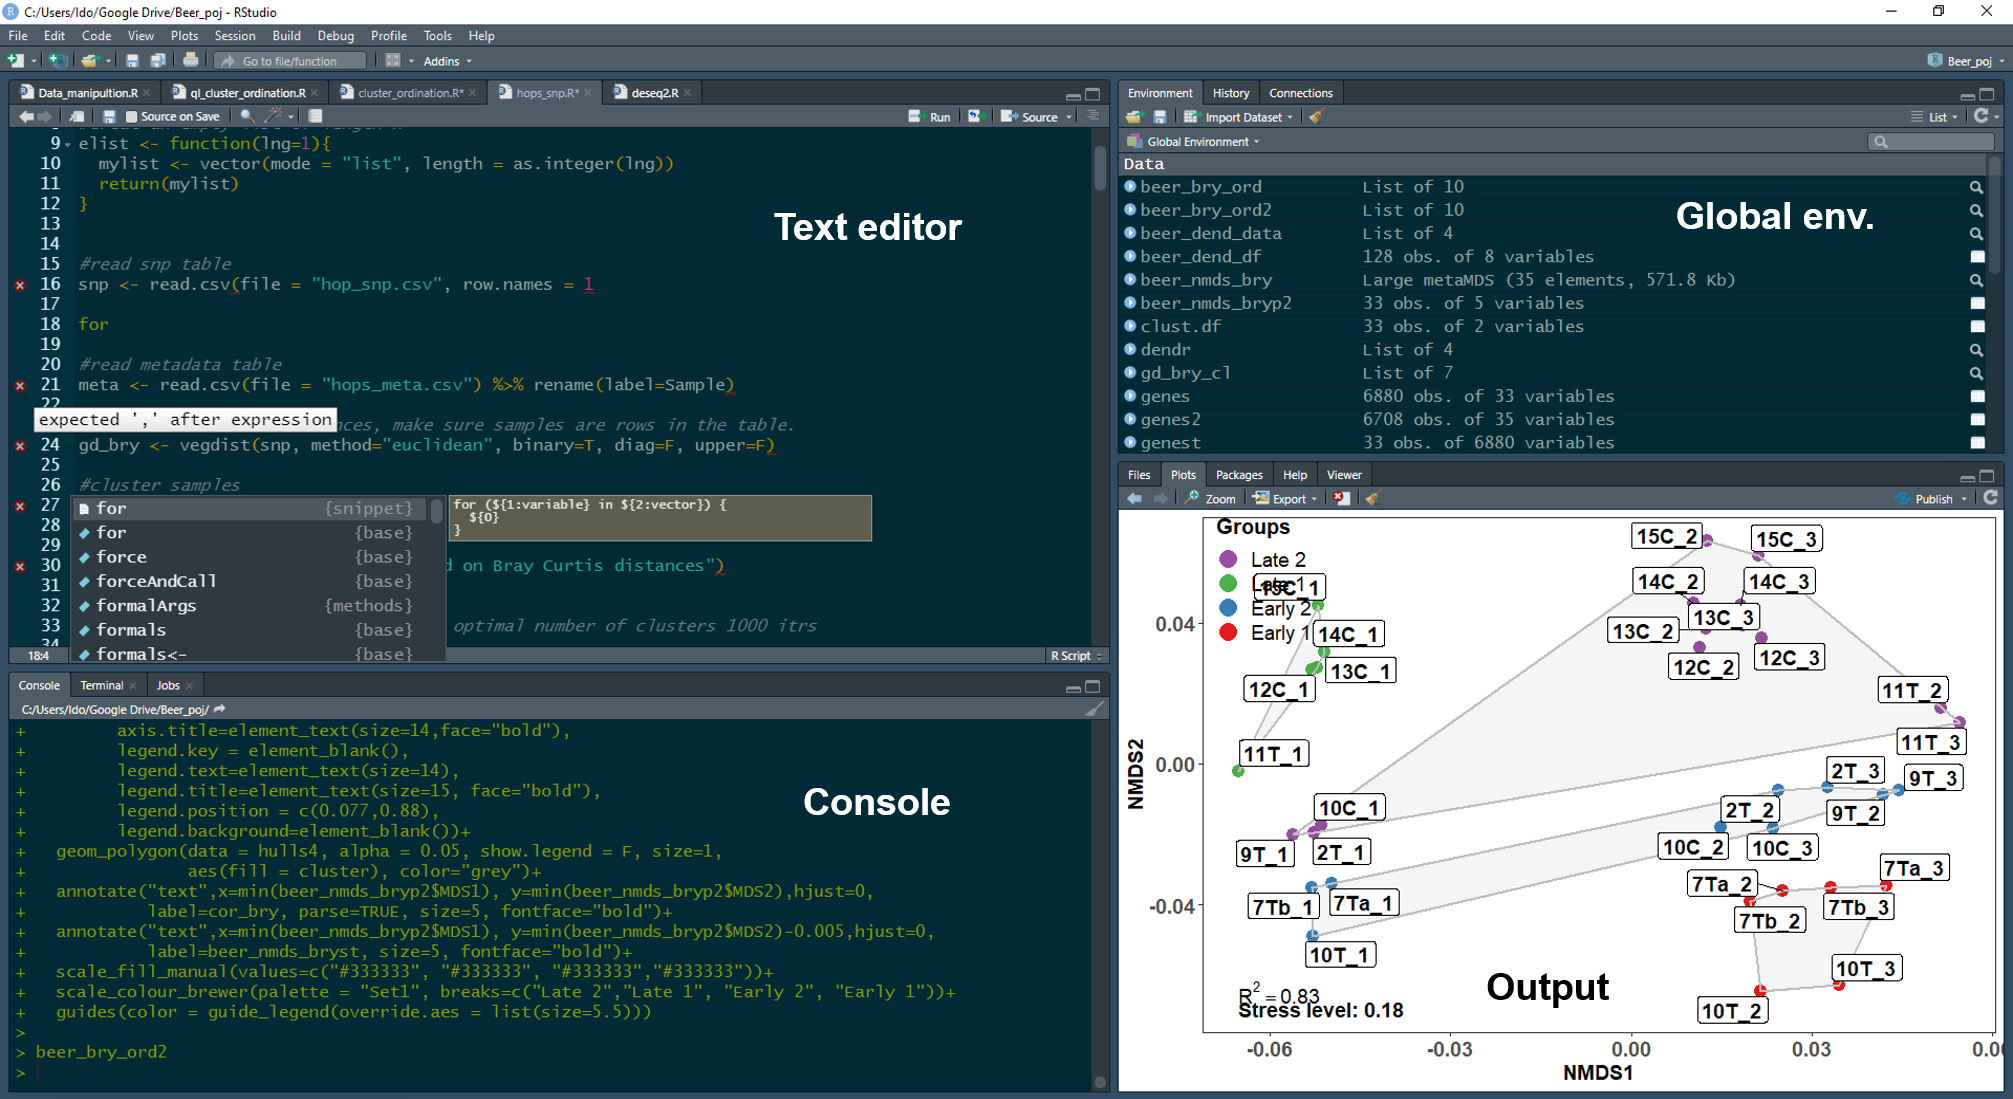
\includegraphics[width=1\linewidth]{figs/Rstudio1} 

}

\end{figure}

Unlike the basic console GUI, RStudio allows you to mange and separate different R project (e.g.~you could have a
separate project for this course and and for a stats course).
Another advantage of R studio is its integration of version control which include both Git and SVG. This will be
beneficial if future course when you will be required to collaborate on projects.

\hypertarget{the-text-editor-pane}{%
\subsubsection*{\texorpdfstring{\textbf{The text editor pane}}{The text editor pane}}\label{the-text-editor-pane}}
\addcontentsline{toc}{subsubsection}{\textbf{The text editor pane}}

The text editor pane is found on the top left corner of the RStudio screen. The text editor allows you to edit code
before sending it to the console. As shown in the figure below, there are some advantages of writing your code with
the RStudio code editor. It auto-completes syntax, functions, and variables. The text editor also helps in code
debugging by flagging lines with errors (marked by a red dot with an X). It also allows you to edit multiple
scripts using tabs, just like your web browser.

\begin{figure}

{\centering 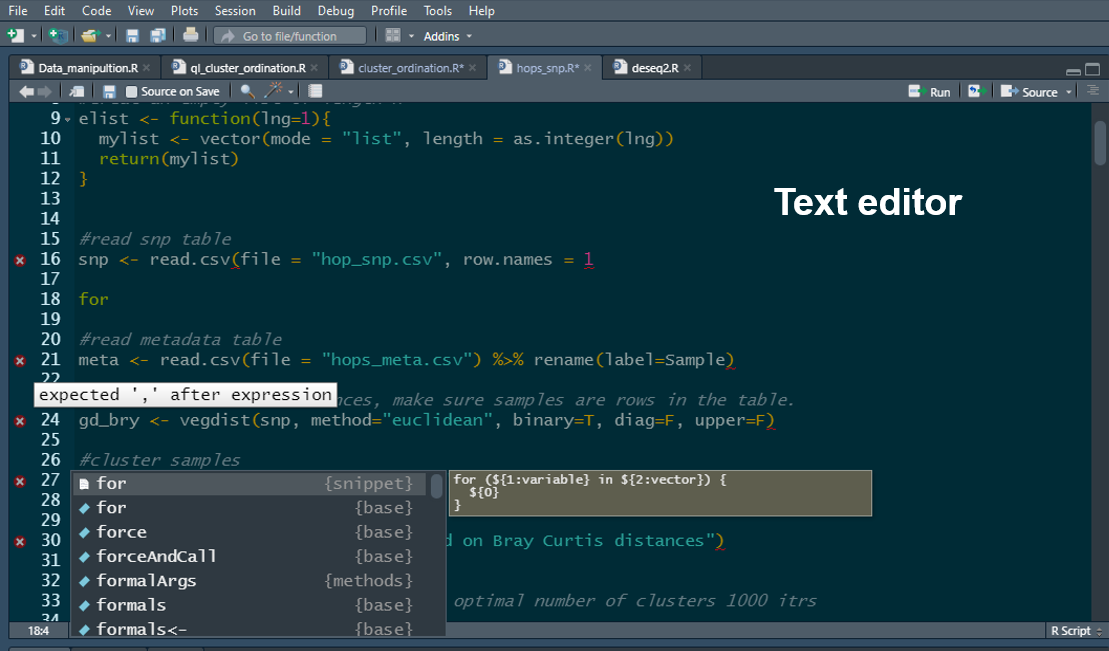
\includegraphics[width=0.8\linewidth]{figs/texteditor} 

}

\caption{The RStudio text editor}\label{fig:unnamed-chunk-6}
\end{figure}

Using the text editor allows you to send code to the console line by line (or as chunks, by highlighting multiple
lines) by using a keyboard shortcut(command enter in mac-OS, Ctrl enter win and Linux).
Alternatively this can also be done pressing the run button at the top left corner of the editor. The editor also
allows you to source the entire script to the console by pressing the source button (the rightmost button).
The text editor supports multiple languages(e.g.~C++, python, SQL, etc\ldots) if you fancy programming in a language
other than R.

\hypertarget{the-console-pane}{%
\subsubsection*{\texorpdfstring{\textbf{The console pane}}{The console pane}}\label{the-console-pane}}
\addcontentsline{toc}{subsubsection}{\textbf{The console pane}}

The console pane is found below the text editor.This is where code input and output resulting from the code can be
seen. You can also write and run code directly at the console, just like when using the R interpreter GUI. The
console allows you to manage multiple R jobs (we will not use that) through the job tab, as well as running a bash
terminal (terminal tab) for system commands (we might use that).

\begin{figure}

{\centering 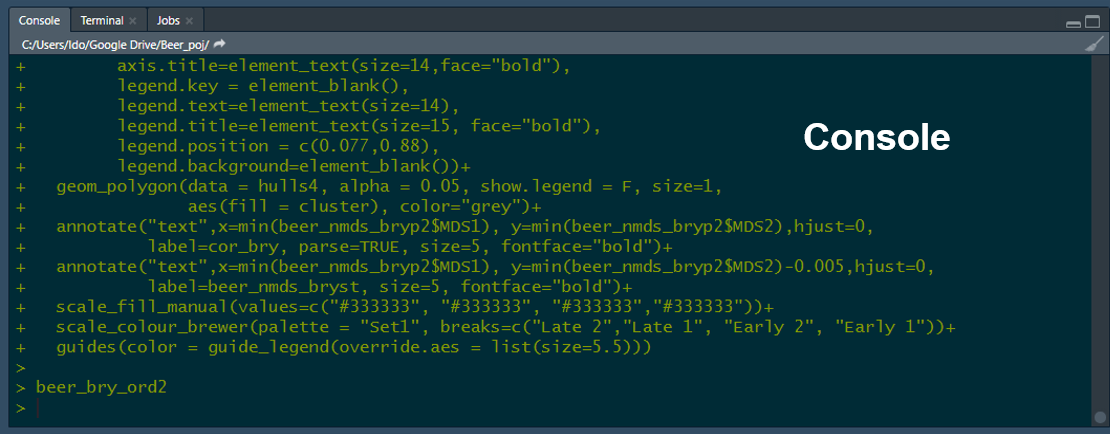
\includegraphics[width=0.8\linewidth]{figs/console} 

}

\caption{The RStudio console}\label{fig:unnamed-chunk-7}
\end{figure}

\hypertarget{the-global-environment-pane}{%
\subsubsection*{\texorpdfstring{\textbf{The global environment pane}}{The global environment pane}}\label{the-global-environment-pane}}
\addcontentsline{toc}{subsubsection}{\textbf{The global environment pane}}

The global environment pane is found to the right of the text editor, this is where you can see all the variables you
called. It will also tell you what type of variables they are and how much memory they use.

\begin{figure}

{\centering 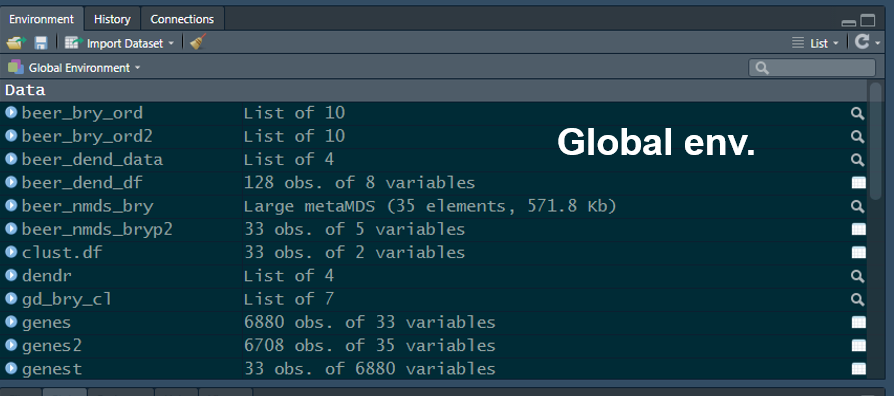
\includegraphics[width=0.8\linewidth]{figs/globenv} 

}

\end{figure}

The global environment pane also contains a history and a connection tab. The history tab saves all the lines of code
ran through the console. It also allows you to resend lines of code back to the text editor which is very useful if
you deleted them by accident instead of commenting them out. The connection tab allows you to connect RStudio to
database servers (e.g.~SQL (ODBC) or Spark, we will not use that).

\hypertarget{the-output-pane}{%
\subsubsection*{\texorpdfstring{\textbf{The output pane}}{The output pane}}\label{the-output-pane}}
\addcontentsline{toc}{subsubsection}{\textbf{The output pane}}

The output pane is found bellow the global environment pane and is where graphical output will show up. Here you can
scroll through as well as export all of the plots that you generated while analyzing data and running scripts.

\begin{figure}

{\centering 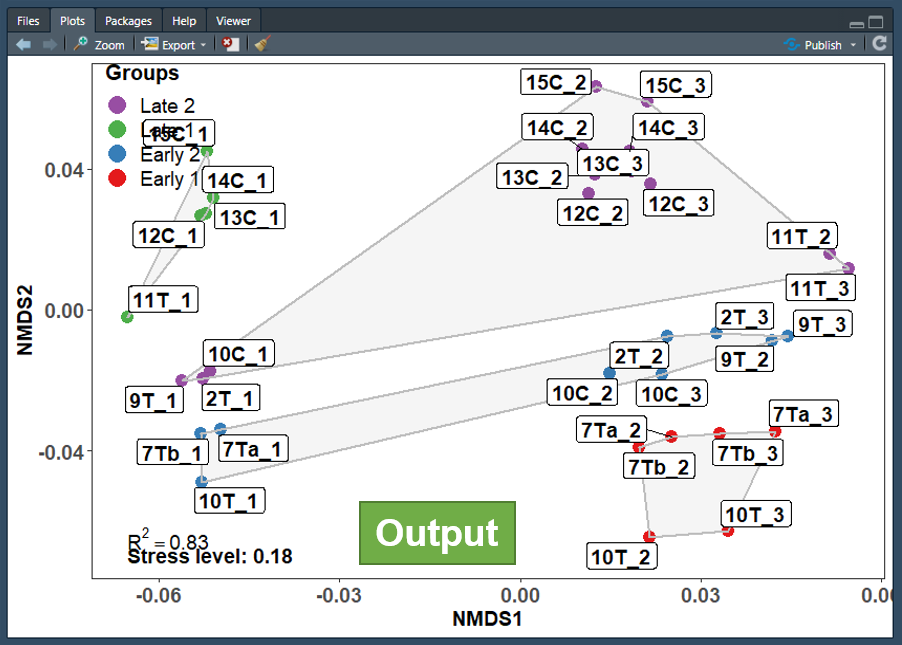
\includegraphics[width=0.8\linewidth]{figs/output} 

}

\end{figure}

The output pane also includes a file tab which allows you to see all the files you exported as well as a help tab
which allows you to brows through documentation with details of the functions you might want to run. The package tab
helps you manage the R extension packages you might have installed and allows you to see which ones are loaded.

\begin{center}\rule{0.5\linewidth}{0.5pt}\end{center}

\begin{quote}
Note that each of these panes include tabs that were not included in this tutorial. However, they can be very
useful and I encourage you to explore them as you learn to use RStudio.
\end{quote}

\begin{center}\rule{0.5\linewidth}{0.5pt}\end{center}

\hypertarget{short-exercise-in-rstudio}{%
\subsubsection*{\texorpdfstring{\textbf{Short exercise in RStudio}}{Short exercise in RStudio}}\label{short-exercise-in-rstudio}}
\addcontentsline{toc}{subsubsection}{\textbf{Short exercise in RStudio}}

Copy the following code to RStudio's text editor

\begin{Shaded}
\begin{Highlighting}[]
\NormalTok{j }\OtherTok{\textless{}{-}} \StringTok{"Harry"}
\NormalTok{k }\OtherTok{\textless{}{-}} \StringTok{"Poter"}
\NormalTok{rowling }\OtherTok{\textless{}{-}} \FunctionTok{data.frame}\NormalTok{(}\AttributeTok{First\_name =}\NormalTok{ j,}\AttributeTok{Last\_name =}\NormalTok{ k)}

\FunctionTok{data}\NormalTok{(cars)}
\NormalTok{car\_data }\OtherTok{\textless{}{-}}\NormalTok{ cars}
\FunctionTok{plot}\NormalTok{(cars)}
\end{Highlighting}
\end{Shaded}

\begin{Shaded}
\begin{Highlighting}[]
\NormalTok{Useless.function }\OtherTok{\textless{}{-}} \ControlFlowTok{function}\NormalTok{(x)\{}
  \ControlFlowTok{if}\NormalTok{(}\FunctionTok{is.numeric}\NormalTok{(x))\{}
  \FunctionTok{print}\NormalTok{(}\StringTok{"This function is goddamn useless"}\NormalTok{)}
\NormalTok{  \} }\ControlFlowTok{else}\NormalTok{ \{}
    \FunctionTok{print}\NormalTok{(}\StringTok{"This function is goddamn useless"}\NormalTok{)}
\NormalTok{  \}}
\NormalTok{\}}
\end{Highlighting}
\end{Shaded}

Try writing the last line instead of copying and pasting it, did you notice how the editor completes the syntax for
you as the function data.frame is called?

Practice running it line by line, as a chunk, and sourcing it completely.

What happens in the global environment when you ran the code?

Are all called variables listed under the same category in the global environment pane?

Can you tell how much memory is car\_data using?

What happens when you press rowling?

What do you see in the output pane?

What happens when you call the rowling variable directly in the console?

\hypertarget{programming-in-r---the-basics}{%
\section*{\texorpdfstring{\textbf{Programming in R - the basics}}{Programming in R - the basics}}\label{programming-in-r---the-basics}}
\addcontentsline{toc}{section}{\textbf{Programming in R - the basics}}

\hypertarget{r-language-and-syntax}{%
\subsection*{\texorpdfstring{\textbf{R language and syntax}}{R language and syntax}}\label{r-language-and-syntax}}
\addcontentsline{toc}{subsection}{\textbf{R language and syntax}}

R is an expression language with very simple syntax requiring that you list call-functions, in order to perform tasks
on your data.

In the code bellow two functions were called, first is the mathematical operator +, this is somewhat of an irregular
function structure ( \href{https://en.wikipedia.org/wiki/Infix_notation}{infix function} if you're interested) that tells
R to sum the two numbers.
In this case, the arguments (the numbers needed to be summed) are placed on both side of the function (again in this
case the + operator). These are referred to as left hand side (LHD) and right hand side (RHD) arguments.
The second function is the print function, which is a regular function, and R syntax
requires that you write the arguments within parenthesis that come after the function.

\begin{Shaded}
\begin{Highlighting}[]
\CommentTok{\#Calling an irregular function \textless{}{-}{-} btw this is how you comment}
\DecValTok{1}\SpecialCharTok{+}\DecValTok{1}
\end{Highlighting}
\end{Shaded}

\begin{verbatim}
## [1] 2
\end{verbatim}

\begin{Shaded}
\begin{Highlighting}[]
\CommentTok{\#Calling a regular function}
\FunctionTok{print}\NormalTok{(j)}
\end{Highlighting}
\end{Shaded}

\begin{verbatim}
## [1] "Harry"
\end{verbatim}

The code snippet above is an example for a script where functions are separated by a line, and each function runs
sequentially. Functions, however, can also be separated by a semicolon (;) and written in the same line as can be
seen in the code snippet bellow. Note that while the example bellow gives identical results this writing style is not
encouraged as it reduces the readability of the code.

\begin{Shaded}
\begin{Highlighting}[]
\CommentTok{\#An example of poor code}
\DecValTok{1}\SpecialCharTok{+}\DecValTok{1}\NormalTok{;}\FunctionTok{print}\NormalTok{(j)}
\end{Highlighting}
\end{Shaded}

\begin{verbatim}
## [1] 2
\end{verbatim}

\begin{verbatim}
## [1] "Harry"
\end{verbatim}

R is case sensitive, whenever a function is called one needs to make sure that
both it and it's arguments are written properly, otherwise the function will produce an error.

\begin{Shaded}
\begin{Highlighting}[]
\CommentTok{\#Variable is capitalized}
\FunctionTok{print}\NormalTok{(J)}
\end{Highlighting}
\end{Shaded}

\begin{verbatim}
## Error in print(J): object 'J' not found
\end{verbatim}

\begin{Shaded}
\begin{Highlighting}[]
\CommentTok{\#Function name is capitalized}
\FunctionTok{Print}\NormalTok{(j)}
\end{Highlighting}
\end{Shaded}

\begin{verbatim}
## Error in Print(j): could not find function "Print"
\end{verbatim}

The print function only accepts one argument, however some functions in R accept multiple arguments. The code bellow
calls the function c, c concatenates similar variables in R into one variable. When more than one
argument is used, the arguments should be separated by a comma (``,'').

\begin{Shaded}
\begin{Highlighting}[]
\CommentTok{\#Spoiler for the order of operations in R}
\FunctionTok{print}\NormalTok{(}\FunctionTok{c}\NormalTok{(j,k))}
\end{Highlighting}
\end{Shaded}

\begin{verbatim}
## [1] "Harry" "Poter"
\end{verbatim}

Here is another example of a function that accepts more than one argument. The sep argument is an example of an
argument that's not a variable.

\begin{Shaded}
\begin{Highlighting}[]
\CommentTok{\#j and k are variables, sep (short for separator) is not.}

\FunctionTok{print}\NormalTok{( }\FunctionTok{paste}\NormalTok{(j,k, }\AttributeTok{sep =} \StringTok{";"}\NormalTok{) )}
\end{Highlighting}
\end{Shaded}

\begin{verbatim}
## [1] "Harry;Poter"
\end{verbatim}

So how can you tell which or how many arguments does a function accept? Well, the RStudio text editor offers a
glimpse of the arguments as you write the function but the proper way to do is is to call the function documentation.
This is done by invoking the help function, which uses the ? operator as seen in the code snippet below.

\begin{Shaded}
\begin{Highlighting}[]
\NormalTok{?paste}

\CommentTok{\# This is equivalent of help(paste)}
\CommentTok{\#? is another irregular function that accepts a LHS argument}
\end{Highlighting}
\end{Shaded}

When running this code using RStudio, the help tab will be prompted and you will be able to see the paste function
documentation. Arguments for the function are specified both under usage and arguments.
Usage specify the arguments and informs the user of arguments with set values, for example the argument sep has a set
value of '' ``, which denotes white space. Often you would encounter arguments with a set value of NULL, this lets R
know that for all intents and purposes the argument should be ignored unless value is specified by the user.\\
The arguments section provides an explanation regarding to the function of each of the arguments. For example the
value sep is a character string that separates the terms being pasted. This means that the default separator for
pasted terms is a white space.

\begin{center}\rule{0.5\linewidth}{0.5pt}\end{center}

\begin{quote}
\textbf{The \ldots{} (dot dot dot) argument}

The paste function also include the ``\ldots{}'' argument, this is a special argument that matches any unspecified
arguments and makes sure that the function accepts them if possible. Here, the underlying conditions is that any
unspecified argument must be a vector (we will discuss what vectors are later in this tutorial).
\end{quote}

\begin{center}\rule{0.5\linewidth}{0.5pt}\end{center}

\textbf{Extended search}

Sometimes the documentation for a function is not found in the environment you loaded (we will get to libraries of
functions extending the capabilities of R later in this tutorial), in order to perform an extended search of all
libraries installed on your computer use double question mark (``??'').

\textbf{Quick R exercise:}

\begin{enumerate}
\def\labelenumi{\arabic{enumi}.}
\tightlist
\item
  The previous code snippets provided a good example of the order of operation in R when nesting functions. Look at the code bellow, what do you think the order of operation is? Which function will run firs? Which will run second, which will run third?
\end{enumerate}

\begin{Shaded}
\begin{Highlighting}[]
\FunctionTok{print}\NormalTok{(}\FunctionTok{paste}\NormalTok{(}\FunctionTok{c}\NormalTok{(j,k), }
            \FunctionTok{c}\NormalTok{(k,j), }\AttributeTok{sep =} \StringTok{" "}\NormalTok{))}
\end{Highlighting}
\end{Shaded}

\begin{enumerate}
\def\labelenumi{\arabic{enumi}.}
\setcounter{enumi}{1}
\tightlist
\item
  sum is a function in R. Can you find its purpose and how many arguments does it accept?
\end{enumerate}

\begin{center}\rule{0.5\linewidth}{0.5pt}\end{center}

\begin{quote}
\textbf{A Note on indentation in R}

The example code above includes indentation however, unlike in other programming languages, R does not require that you indent your code. Indentation is only used to make code more readable to humans, especially as it gets more complex. As you will learn, the flow of operations in the basic R is determined by parenthesis ``()'' when combining functions (e.g.~the code above) and braces ``\{\}'' when writing costume functions and statements (an example of that is the Useless.function).
\end{quote}

\begin{center}\rule{0.5\linewidth}{0.5pt}\end{center}

\#\# \textbf{Expanding R's capabilities by installing additional function packages}

The R language includes an extensive array of functions. Those are known as base R, or core R functions. However,
sometimes developers will write R functions that enhance R's capabilities beyond the scope of the basic core
functions (e.g.~enhanced graphical capabilities, faster and more efficient data manipulation, etc.) or functions
designed for a specialized tasks which doesn't concern most R users (e.g.~population genetics, SQL integration etc.).

Usually developers package their functions in what is known as function libraries, or packages, and publish them to
the public. These packages can be downloaded and installed by R users, and the functions they contain expand the
capabilities of R.

There are several repositories that store R packages, here we will go over 3 of them.

\begin{enumerate}
\def\labelenumi{\arabic{enumi}.}
\tightlist
\item
  \textbf{The CRAN repository:}
\end{enumerate}

The \href{https://cran.r-project.org/web/packages/available_packages_by_name.html}{CRAN repository} is the main repository for R packages. It is maintained and rigorously curated by the R foundation and currently contains over 15K packages. The scope of these packages is very broad and they can enhance R capabilities in anything from graphical representation of data, to genomic analysis, to development of web applications. Each of the packages featured in the CRAN repository contains documentations including a manual with a list of all functions included in the package and examples for how to use them. Some contain workflows.

To install a package from the CRAN repository use the function install.packages, note that install.packages doesn't load the package. If you want to call functions from within this package you need to load it using the function library ().
Alternatively you can use ``::'' which allows you to call the function without load the package that contains it. This may also be used if you loaded two packages that contain a function with similar name, or if a function from one package is masking another.

\begin{Shaded}
\begin{Highlighting}[]
\CommentTok{\#note the use of \textquotesingle{}\textquotesingle{} around the argument in these functions, they will recognize the argument without the use of \textquotesingle{} \textquotesingle{} however it is considered good practice to write the code with them.}

\FunctionTok{install.packages}\NormalTok{(}\StringTok{\textquotesingle{}x\textquotesingle{}}\NormalTok{)}
\FunctionTok{library}\NormalTok{(}\StringTok{\textquotesingle{}x\textquotesingle{}}\NormalTok{)}
\NormalTok{x}\SpecialCharTok{::}\FunctionTok{function.x}\NormalTok{()}
\end{Highlighting}
\end{Shaded}

\begin{enumerate}
\def\labelenumi{\arabic{enumi}.}
\setcounter{enumi}{1}
\tightlist
\item
  \textbf{Bioconductor:}
\end{enumerate}

\href{}{Bioconductor} is a repository for packages designed for handle and analyse high throughput biological data (e.g.~omics, flow cytometry, etc.). Contains over 1800 packages, however not all packages aimed at analyzing high throughput biological data are published in Bioconductor since it requires the variables to be stored in an object with specialized structure (S4 object). The packages are curated by the Bioconductor project for open source bioinformatic software. Each Bioconductor package contains at least one vignette, a document that provides a task-oriented description of package functionality. Most also contains a manual with example SOPs.

\begin{enumerate}
\def\labelenumi{\arabic{enumi}.}
\setcounter{enumi}{2}
\tightlist
\item
  \textbf{GitHub:}
\end{enumerate}

GitHab is basically a developer's domain, and most if not all R packages are stored on GitHab at one point or another
during the stage for their development. Most packages also have a GitHub version in addition to the CRAN or
Bioconductor version. The version on GitHub is a developer version with capabilities absent from the official
distribution of the package. Those versions are normally less stable as they are in the testing stage of the
development. There is no curation of github packages, therefore documentation is patchy.

Installing packages from Bioconductor and GitHub require additional package managers and have their own special
installation functions. We will go over it during labs 3-4.

\begin{center}\rule{0.5\linewidth}{0.5pt}\end{center}

\textbf{Quick R exercise}

\begin{enumerate}
\def\labelenumi{\arabic{enumi}.}
\item
  Install the package vegan from the CRAN repository
\item
  What is the purpose of this package?
\item
  How many arguments does the anosim function from this package accepts, how many of them are variables?
\end{enumerate}

\begin{center}\rule{0.5\linewidth}{0.5pt}\end{center}

\hypertarget{variable-assignment-in-r---vs---vs}{%
\section{\texorpdfstring{\textbf{Variable assignment in R (\textless- vs -\textgreater{} vs =)}}{Variable assignment in R (\textless- vs -\textgreater{} vs =)}}\label{variable-assignment-in-r---vs---vs}}

R has three ways of assigning values to variables, two of them are leftwards and one rightwards.
Leftwards assignment is the most common way to assign value to variables, this is similar to other programming language like python or C++. In R this is achieved by using the assign operator ``\textless-'', or alternatively similar to python and C++ by using the equal operator ``=''.

Leftwards assignment groups the values from right to left, therefore in the snippet bellow the value of the variable v will be 1 and the value of of variable v2 will also be 1 since it will get the value of variable v.

While on the surface both methods work identically, beneath the surface they are quit different and using ``='' may lead to errors . Therefore, the convention is to always use ``\textless-'' over ``=''.

\begin{Shaded}
\begin{Highlighting}[]
\CommentTok{\#This is leftwards assignment}
\NormalTok{v }\OtherTok{\textless{}{-}} \DecValTok{1}

\CommentTok{\#This is an alternative leftwards assignment}

\NormalTok{v2 }\OtherTok{=}\NormalTok{ v}

\NormalTok{v}
\end{Highlighting}
\end{Shaded}

\begin{verbatim}
## [1] 1
\end{verbatim}

\begin{Shaded}
\begin{Highlighting}[]
\NormalTok{v2}
\end{Highlighting}
\end{Shaded}

\begin{verbatim}
## [1] 1
\end{verbatim}

Rightwards assignment works opposite to leftwards assignment. It uses the rightwards assign operator ``-\textgreater{}'', and groups
everything left to right. Therefore, in the code snippet bellow, the value of variable v2 will now be 3. Note that
rightwards assignment is discouraged and good coding practices dictate that all variables should be assigned using
the leftwards method.

\begin{Shaded}
\begin{Highlighting}[]
\DecValTok{3} \OtherTok{{-}\textgreater{}}\NormalTok{ v2}

\NormalTok{v}
\end{Highlighting}
\end{Shaded}

\begin{verbatim}
## [1] 1
\end{verbatim}

\begin{Shaded}
\begin{Highlighting}[]
\NormalTok{v2}
\end{Highlighting}
\end{Shaded}

\begin{verbatim}
## [1] 3
\end{verbatim}

\begin{center}\rule{0.5\linewidth}{0.5pt}\end{center}

\begin{quote}
\textbf{A note on alliasing and R}

While the code above assigns the value of v to variable v2. Unlike in python or java for example, this does not
create an alias (creating an alternative name for a variable stored in memory) and there is no link between v and
v2. v2 can be assigned a different value or be edited by upending more values to it or modifying the original value
and v1 will not be affected.
\end{quote}

\begin{center}\rule{0.5\linewidth}{0.5pt}\end{center}

\hypertarget{rules-for-variable-naming-in-r}{%
\section{\texorpdfstring{\textbf{Rules for variable naming in R}}{Rules for variable naming in R}}\label{rules-for-variable-naming-in-r}}

Variable naming in R follows a few simple rules:

\begin{itemize}
\item
  Variable names must not be the same as R's special characters or functions (except for c)
\item
  Variable names must always start with a letter, however they may contain numbers and other characters
\item
  Special characters must be escaped using ``, and it is recommended that they be avoided in general
\item
  Variable names are case sensitive (but you already know that)
\end{itemize}

\hypertarget{data-types-objects-in-r}{%
\chapter{\texorpdfstring{\textbf{Data types (objects) in R}}{Data types (objects) in R}}\label{data-types-objects-in-r}}

The R language has multiple classes of data types often referred to as objects, though R is not an object oriented
programming language per se. Those include but not limited to vectors, lists, matrices, and data.frames. Each of
these is optimized to handle either single or multidimensional information and is part of what makes R such a
powerful tool in handling, analyzing, and representing data. This part will go over the commonly used data types in
R.

\hypertarget{atomic-vectors}{%
\section{\texorpdfstring{\textbf{``Atomic'' vectors}}{``Atomic'' vectors}}\label{atomic-vectors}}

Atomic vectors are probably the most basic form of data class in R. Similar to lists in python, they contain a
sequence of elements. In fact, the output from all the functions used in this tutorial so far were vectors with one
element. That is the reason {[}1{]} was displayed next to the output, to denote the first element in the vector. In R,
each atomic vector class is capable of only storing information of the same type. There are four main classes of
atomic vectors in R, this part will detail them and how to work with them.

\hypertarget{numeric-vectors-double-and-integer}{%
\subsection{\texorpdfstring{\textbf{Numeric vectors (double and integer):}}{Numeric vectors (double and integer):}}\label{numeric-vectors-double-and-integer}}

Numeric vectors store elements that are numbers, R has two common classes of numeric vectors: double (double precision \href{https://en.wikipedia.org/wiki/Floating-point_arithmetic}{folating point numbers}) and integer.

The easiest way to create a numeric vector is using the function c which you have already encountered.

\begin{Shaded}
\begin{Highlighting}[]
\CommentTok{\#double}
\NormalTok{dub.vec }\OtherTok{\textless{}{-}} \FunctionTok{c}\NormalTok{(}\DecValTok{1}\NormalTok{,}\DecValTok{2}\NormalTok{,}\DecValTok{3}\NormalTok{)}

\CommentTok{\#integer}
\NormalTok{int.vec }\OtherTok{\textless{}{-}} \FunctionTok{c}\NormalTok{(1L,2L,3L)}

\CommentTok{\#alt way to get an interger sequence, : tells R to get all natural numbers between 1 and 3 }

\NormalTok{int.vec2 }\OtherTok{\textless{}{-}}\NormalTok{ (}\DecValTok{1}\SpecialCharTok{:}\DecValTok{3}\NormalTok{)}


\NormalTok{dub.vec}
\end{Highlighting}
\end{Shaded}

\begin{verbatim}
## [1] 1 2 3
\end{verbatim}

\begin{Shaded}
\begin{Highlighting}[]
\NormalTok{int.vec}
\end{Highlighting}
\end{Shaded}

\begin{verbatim}
## [1] 1 2 3
\end{verbatim}

\begin{Shaded}
\begin{Highlighting}[]
\CommentTok{\#Note this is one way of comparing variables in R}
\NormalTok{dub.vec }\SpecialCharTok{==}\NormalTok{ int.vec}
\end{Highlighting}
\end{Shaded}

\begin{verbatim}
## [1] TRUE TRUE TRUE
\end{verbatim}

Because the snippet above uses \href{https://en.wikipedia.org/wiki/Natural_number}{natural numbers}, the output of the two
vectors is pretty much identical (as demonstrated by the is.equal operator ``==''). Furthermore, as will be detailed
later, regardless of the type of numbers used, R will automatically convert classes of numeric vectors when needed.
However, sometimes it might behoove you know whether a vector contains floats or integers. The RStudio global
environment pane will denote if a vector is a number or integer, however a more R way to do it is to use the function
typeof().

\begin{Shaded}
\begin{Highlighting}[]
\FunctionTok{typeof}\NormalTok{(dub.vec)}
\end{Highlighting}
\end{Shaded}

\begin{verbatim}
## [1] "double"
\end{verbatim}

\begin{Shaded}
\begin{Highlighting}[]
\FunctionTok{typeof}\NormalTok{(int.vec)}
\end{Highlighting}
\end{Shaded}

\begin{verbatim}
## [1] "integer"
\end{verbatim}

Working with numerical vectors is pretty straightforward, R allows you to perform mathematical operations on them,
sum them and even concatenate them. When concatenating an integer and double to a single vector R will coarse it to
double. This is because coercing a float to integer will result in dropping the float (i.e.~4.99 will be coerced to 4
you can try it using as.integer(4.99) ). Therefore coercing to double is less restrictive.

\begin{Shaded}
\begin{Highlighting}[]
\CommentTok{\#concatenating vactors plus a bonus example of nesting functions. }
\CommentTok{\#note that you can use the assign operator within a function, that\textquotesingle{}s one of the differences }
\CommentTok{\#between it and using "=" .}
\FunctionTok{typeof}\NormalTok{(num.vec }\OtherTok{\textless{}{-}} \FunctionTok{c}\NormalTok{(dub.vec,int.vec))}
\end{Highlighting}
\end{Shaded}

\begin{verbatim}
## [1] "double"
\end{verbatim}

\begin{Shaded}
\begin{Highlighting}[]
\NormalTok{num.vec}
\end{Highlighting}
\end{Shaded}

\begin{verbatim}
## [1] 1 2 3 1 2 3
\end{verbatim}

\begin{Shaded}
\begin{Highlighting}[]
\CommentTok{\#note how when performing a mathematical operation on a vector it is perfomed individually on all}
\CommentTok{\#the ellements of the vector, negating the need to use a for loop. Flanking the operation with () serves as a call for the newly created variable.}

\NormalTok{(sq.num.vec }\OtherTok{\textless{}{-}}\NormalTok{ num.vec}\SpecialCharTok{\^{}}\DecValTok{2}\NormalTok{)}
\end{Highlighting}
\end{Shaded}

\begin{verbatim}
## [1] 1 4 9 1 4 9
\end{verbatim}

\hypertarget{indexing-and-subseting-numeric-vectors}{%
\subsection{\texorpdfstring{\textbf{Indexing and subseting numeric vectors}}{Indexing and subseting numeric vectors}}\label{indexing-and-subseting-numeric-vectors}}

R makes it easy to index, access and subset every element of a numeric vector, this is done using the square brackets. One thing to note is that unlike non-math programming language (looking at you python), R starts indexing at 1 and not at 0.

In the example below, I used the function rnorm to generate a vector of 100 random numbers normally distributed around a mean of 45 (which would probably be the average for this course) and a standard deviation of 18.

\begin{Shaded}
\begin{Highlighting}[]
\CommentTok{\#Note how I didn\textquotesingle{}t specefy the arguments, R knows to match them }
\CommentTok{\#you just have to make sure you write them in the correct order.}
\NormalTok{this.course.avarage }\OtherTok{\textless{}{-}} \FunctionTok{round}\NormalTok{(}\FunctionTok{rnorm}\NormalTok{(}\DecValTok{100}\NormalTok{, }\DecValTok{45}\NormalTok{, }\DecValTok{18}\NormalTok{),}\DecValTok{2}\NormalTok{)}

\CommentTok{\#We can see if our vector is indeed 100 elements long using the function length}

\FunctionTok{length}\NormalTok{(this.course.avarage)}
\end{Highlighting}
\end{Shaded}

\begin{verbatim}
## [1] 100
\end{verbatim}

\begin{Shaded}
\begin{Highlighting}[]
\CommentTok{\#Head lets you glimps the first n elements in a variable, default is 6 (tail is for last)}
\FunctionTok{head}\NormalTok{(this.course.avarage)}
\end{Highlighting}
\end{Shaded}

\begin{verbatim}
## [1] 56.68 38.81 42.88 27.53 44.56 44.18
\end{verbatim}

\begin{Shaded}
\begin{Highlighting}[]
\CommentTok{\#You can access any element on the vector using the square brackets[]}
\CommentTok{\#lets acces the first 10 elements in the vector}
\NormalTok{this.course.avarage[}\DecValTok{1}\SpecialCharTok{:}\DecValTok{10}\NormalTok{]}
\end{Highlighting}
\end{Shaded}

\begin{verbatim}
##  [1] 56.68 38.81 42.88 27.53 44.56 44.18 32.01 83.74 47.82 33.47
\end{verbatim}

\begin{Shaded}
\begin{Highlighting}[]
\CommentTok{\#You can also replace them with whatever it is you want, lets replace the first 10 elements with a copy of the last 10 elements.}

\NormalTok{this.course.avarage[}\DecValTok{1}\SpecialCharTok{:}\DecValTok{10}\NormalTok{] }\OtherTok{\textless{}{-}}\NormalTok{ this.course.avarage[}\DecValTok{91}\SpecialCharTok{:}\DecValTok{100}\NormalTok{]}

\NormalTok{this.course.avarage[}\DecValTok{1}\SpecialCharTok{:}\DecValTok{10}\NormalTok{]}
\end{Highlighting}
\end{Shaded}

\begin{verbatim}
##  [1] 20.87 39.93 78.75 38.11 30.94 47.42 29.13 58.48 37.08 30.92
\end{verbatim}

\begin{Shaded}
\begin{Highlighting}[]
\NormalTok{this.course.avarage[}\DecValTok{91}\SpecialCharTok{:}\DecValTok{100}\NormalTok{]}
\end{Highlighting}
\end{Shaded}

\begin{verbatim}
##  [1] 20.87 39.93 78.75 38.11 30.94 47.42 29.13 58.48 37.08 30.92
\end{verbatim}

\begin{Shaded}
\begin{Highlighting}[]
\FunctionTok{length}\NormalTok{(this.course.avarage)}
\end{Highlighting}
\end{Shaded}

\begin{verbatim}
## [1] 100
\end{verbatim}

\begin{Shaded}
\begin{Highlighting}[]
\CommentTok{\#note that indexing and subseting works in reverse order too}
\NormalTok{another.course.avarage }\OtherTok{\textless{}{-}} \FunctionTok{c}\NormalTok{(this.course.avarage[}\DecValTok{1}\SpecialCharTok{:}\DecValTok{5}\NormalTok{],this.course.avarage[}\DecValTok{25}\SpecialCharTok{:}\DecValTok{20}\NormalTok{])}

\CommentTok{\#What would the length of this vector be?}

\CommentTok{\#Another great aspect of vectors is that they allow you to change only a subset values without resorting to conditional statments (if else)}

\CommentTok{\#Let\textquotesingle{}s creat a new vector}

\NormalTok{another.course.avarage2 }\OtherTok{\textless{}{-}} \FunctionTok{rnorm}\NormalTok{(}\AttributeTok{n=}\DecValTok{100}\NormalTok{,}\AttributeTok{mean=}\DecValTok{75}\NormalTok{,}\AttributeTok{sd=}\DecValTok{5}\NormalTok{)}

\CommentTok{\#Let\textquotesingle{}s access only marks higher than the avarage}
\NormalTok{another.course.avarage2[another.course.avarage2}\SpecialCharTok{\textgreater{}}\DecValTok{75}\NormalTok{]}
\end{Highlighting}
\end{Shaded}

\begin{verbatim}
##  [1] 81.27745 79.55160 80.81661 76.64541 75.34353 76.35146 77.95521 76.45099
##  [9] 77.63120 75.42647 78.75686 76.72255 78.22906 77.39144 76.51825 79.00782
## [17] 75.10254 80.13483 76.92792 78.93757 75.03633 77.77138 80.27029 75.78761
## [25] 77.19454 76.01650 79.29591 76.71471 80.53481 75.44010 79.22238 78.87174
## [33] 78.51537 79.22241 82.96653 85.46386 80.72279 75.92532 76.69970 78.86211
## [41] 77.66545 84.69615 75.12735 79.38274 82.17418 78.42267 76.76462 80.89843
## [49] 76.14911 77.37502 77.05470
\end{verbatim}

\begin{Shaded}
\begin{Highlighting}[]
\CommentTok{\#lets change anything equal to or grater than the 75 precentile to 100}
\CommentTok{\#this can be done using the quantile function and subseting the 3 element of the vector it produces which it the 75 precentile}
\NormalTok{another.course.avarage2[another.course.avarage2 }\SpecialCharTok{\textgreater{}=} \FunctionTok{quantile}\NormalTok{(another.course.avarage2)[}\DecValTok{3}\NormalTok{]] }\OtherTok{\textless{}{-}} \DecValTok{100}
\NormalTok{another.course.avarage2[another.course.avarage2}\SpecialCharTok{==}\DecValTok{100}\NormalTok{]}
\end{Highlighting}
\end{Shaded}

\begin{verbatim}
##  [1] 100 100 100 100 100 100 100 100 100 100 100 100 100 100 100 100 100 100 100
## [20] 100 100 100 100 100 100 100 100 100 100 100 100 100 100 100 100 100 100 100
## [39] 100 100 100 100 100 100 100 100 100 100 100 100
\end{verbatim}

\begin{center}\rule{0.5\linewidth}{0.5pt}\end{center}

\begin{quote}
\textbf{Quick note on reproducibility}
\end{quote}

\begin{quote}
Note that the numbers generated by the code snippet above will change every time you run it.
This is due to the way random numbers (more accurately \href{https://en.wikipedia.org/wiki/Pseudorandom_number_generator}{pseudorandom numbers}) are generated by ``random'' number generating
algorithms.
If you want to make sure that your code is reproducible you need to set the \href{https://en.wikipedia.org/wiki/Random_seed}{seed} that initializes the pseudorandom number generating algorithm rather than allowing it to be set randomly.
You can do it by incorporating the function set.seed() before you generate numbers, you can use any integer between
the brackets.
\end{quote}

\begin{center}\rule{0.5\linewidth}{0.5pt}\end{center}

\begin{center}\rule{0.5\linewidth}{0.5pt}\end{center}

\textbf{Quick R exercise:}

\begin{enumerate}
\def\labelenumi{\arabic{enumi}.}
\item
  Use the function seq to create a numeric vector of all the natural numbers between 1 and 10.
  If you are unsure of how to use seq, use the help function.
\item
  What type of a numeric vector is the vector you created?
\item
  Create another numeric vector of 10 random elements between 1 and 10 using the function runif()
\item
  What type of a numeric vector did it create?
\item
  Create a third vector by multiplying your first vector by the second vector
\item
  Call the new vector, what can you tell of the order of operations when multiplying vectors in R?
\item
  Replace the 7th element of the first vector, the 8th element of the second vector and the 1st element of the third vector.
\item
  Create a new vector with the final element being -8, the first element being the 7th element of the third vector, the second element being the 5th element of the first vector and the third element being the first element of the
\end{enumerate}

\begin{center}\rule{0.5\linewidth}{0.5pt}\end{center}

\hypertarget{character-vectors}{%
\subsection{\texorpdfstring{\textbf{Character vectors:}}{Character vectors:}}\label{character-vectors}}

Character vectors only store elements that are characters. These could be letters,numbers, or characters. In order for any of those to count as a character it needs to be flanked by double quotation mark (e.g ``j'').

\begin{Shaded}
\begin{Highlighting}[]
\CommentTok{\#Here is how you create a character vector}
\NormalTok{char.vec }\OtherTok{\textless{}{-}} \FunctionTok{c}\NormalTok{(}\StringTok{"a"}\NormalTok{,}\StringTok{"abc"}\NormalTok{,}\StringTok{"abcd"}\NormalTok{)}

\CommentTok{\#Note the length of this vector is 4, the length of each string of characters doesn\textquotesingle{}t impact the }
\CommentTok{\#length of the vector}

\FunctionTok{length}\NormalTok{(char.vec)}
\end{Highlighting}
\end{Shaded}

\begin{verbatim}
## [1] 3
\end{verbatim}

\begin{Shaded}
\begin{Highlighting}[]
\CommentTok{\#Character vectors can contain numbers too}
\NormalTok{char.vec2 }\OtherTok{\textless{}{-}} \FunctionTok{c}\NormalTok{(}\StringTok{"1"}\NormalTok{,}\StringTok{"2"}\NormalTok{,}\StringTok{"3"}\NormalTok{)}
\FunctionTok{typeof}\NormalTok{(char.vec2)}
\end{Highlighting}
\end{Shaded}

\begin{verbatim}
## [1] "character"
\end{verbatim}

\begin{Shaded}
\begin{Highlighting}[]
\CommentTok{\#Tip, R can convert this to a numeric vector}
\CommentTok{\#There is an as.x function for almost every data type in R }
\CommentTok{\#(e.g. as.numeric, as.double, as.character, etc.)}
\NormalTok{char.vec2b }\OtherTok{\textless{}{-}} \FunctionTok{as.numeric}\NormalTok{(char.vec2)}

\CommentTok{\#When concatenating a character and a numeric vector, R will coerce the numeric vector to character.}
\NormalTok{char.vec3 }\OtherTok{\textless{}{-}} \FunctionTok{c}\NormalTok{(char.vec2,int.vec)}
\FunctionTok{typeof}\NormalTok{(char.vec3)}
\end{Highlighting}
\end{Shaded}

\begin{verbatim}
## [1] "character"
\end{verbatim}

\begin{Shaded}
\begin{Highlighting}[]
\CommentTok{\#alternatively you can use the class, class will not differentiate }
\CommentTok{\#between the different numeric vectors but will between the different types of vectors}
\FunctionTok{class}\NormalTok{(char.vec3)}
\end{Highlighting}
\end{Shaded}

\begin{verbatim}
## [1] "character"
\end{verbatim}

\begin{Shaded}
\begin{Highlighting}[]
\CommentTok{\#If you need to generate a sequence of letters from a{-}z}
\NormalTok{char.vec4 }\OtherTok{\textless{}{-}}\NormalTok{ letters[}\DecValTok{1}\SpecialCharTok{:}\DecValTok{7}\NormalTok{]}
\end{Highlighting}
\end{Shaded}

Indexing character vectors is done similarly to numeric vectors

\begin{Shaded}
\begin{Highlighting}[]
\NormalTok{char.vec[}\DecValTok{1}\NormalTok{]}
\end{Highlighting}
\end{Shaded}

\begin{verbatim}
## [1] "a"
\end{verbatim}

\begin{Shaded}
\begin{Highlighting}[]
\CommentTok{\#replacing the first element}
\NormalTok{char.vec[}\DecValTok{1}\NormalTok{] }\OtherTok{\textless{}{-}} \StringTok{"aa"}

\NormalTok{char.vec[}\DecValTok{1}\NormalTok{]}
\end{Highlighting}
\end{Shaded}

\begin{verbatim}
## [1] "aa"
\end{verbatim}

\begin{Shaded}
\begin{Highlighting}[]
\CommentTok{\#adding a fourth element}
\NormalTok{char.vec[}\DecValTok{4}\NormalTok{] }\OtherTok{\textless{}{-}} \StringTok{"Fourth"}

\NormalTok{char.vec[}\DecValTok{4}\NormalTok{]}
\end{Highlighting}
\end{Shaded}

\begin{verbatim}
## [1] "Fourth"
\end{verbatim}

\begin{Shaded}
\begin{Highlighting}[]
\CommentTok{\#To count the number of characters in each of the strings you can use the function nchar}
\FunctionTok{nchar}\NormalTok{(char.vec)}
\end{Highlighting}
\end{Shaded}

\begin{verbatim}
## [1] 2 3 4 6
\end{verbatim}

\begin{Shaded}
\begin{Highlighting}[]
\CommentTok{\#just like with numerical vercots it is possible to subset by value}
\NormalTok{char.vec[char.vec}\SpecialCharTok{==}\StringTok{"a"}\NormalTok{]}
\end{Highlighting}
\end{Shaded}

\begin{verbatim}
## character(0)
\end{verbatim}

\begin{Shaded}
\begin{Highlighting}[]
\CommentTok{\#or rplace a value}
\NormalTok{char.vec[char.vec}\SpecialCharTok{==}\StringTok{"a"}\NormalTok{] }\OtherTok{\textless{}{-}} \StringTok{"a2"}
\end{Highlighting}
\end{Shaded}

\begin{center}\rule{0.5\linewidth}{0.5pt}\end{center}

\textbf{Quick R exercise:}

\begin{enumerate}
\def\labelenumi{\arabic{enumi}.}
\item
  Use R to calculate the total number of character in char.vec (avoid hard coding)
\item
  Use indexing to change the 4th character in the string occupying the 4th element in the vector char.vec with the letter ``B'', no hard coding. Did it work?
\end{enumerate}

\begin{center}\rule{0.5\linewidth}{0.5pt}\end{center}

\begin{quote}
\textbf{A note on working with strings in R}

As you notice in the exercise, indexing a character vector is not the same as indexing the strings that make each
element of the vector. This does not mean that strings are immutable, R has a lot of tools in its arsenal geared
towards manipulating strings. While the future labs will deal with handling biological strings, this is a good
opportunity to look at how R handles strings in general.
Base R has functions such as grep, substring and gsup that work the same way grep in bash works, however, I find the
stringr package much more useful and intuitive.
You can download a cheatsheet guide to stringer \href{https://rstudio.com/resources/cheatsheets/}{here}

Lets look at an example for the capabilities of stringer
\end{quote}

\begin{Shaded}
\begin{Highlighting}[]
\CommentTok{\#load the package you can install it from the cran repo with install.packages}
\FunctionTok{library}\NormalTok{(stringr)}
\NormalTok{borring }\OtherTok{\textless{}{-}} \StringTok{"It was the best of times it was the worst of time"}

\CommentTok{\#count the number of characters}
\FunctionTok{str\_count}\NormalTok{(borring)}
\end{Highlighting}
\end{Shaded}

\begin{verbatim}
## [1] 49
\end{verbatim}

\begin{Shaded}
\begin{Highlighting}[]
\CommentTok{\#split the string in boring to several elelements after every space}
\CommentTok{\#the indexing here is for a list, we will discuss lists later in this lab}

\NormalTok{borring2 }\OtherTok{\textless{}{-}} \FunctionTok{str\_split}\NormalTok{(borring, }\StringTok{" "}\NormalTok{)[[}\DecValTok{1}\NormalTok{]] }\CommentTok{\#note how whitespace is reffered to }

\CommentTok{\#replace a part of a string, lets correct the typo at the end of the sentence to times}

\NormalTok{borring }\OtherTok{\textless{}{-}} \FunctionTok{str\_replace}\NormalTok{(borring, }\StringTok{"time$"}\NormalTok{, }\StringTok{"times"}\NormalTok{) }\CommentTok{\#$ is a regular expression that matches the end of the string, otherwise it would just replace the first time occurrence}
\NormalTok{borring}
\end{Highlighting}
\end{Shaded}

\begin{verbatim}
## [1] "It was the best of times it was the worst of times"
\end{verbatim}

\begin{Shaded}
\begin{Highlighting}[]
\CommentTok{\#How many times does the word it appear in the string? }
\CommentTok{\#Note that R is case sensitive, (?i) searches in a case insensitive way (another regular expression) }

\FunctionTok{str\_count}\NormalTok{(borring, }\StringTok{"(?i)it"}\NormalTok{)}
\end{Highlighting}
\end{Shaded}

\begin{verbatim}
## [1] 2
\end{verbatim}

\begin{quote}
\end{quote}

\begin{center}\rule{0.5\linewidth}{0.5pt}\end{center}

\begin{center}\rule{0.5\linewidth}{0.5pt}\end{center}

\textbf{Quick R exercise:}

Now lets do something a bit biological
Download the stringr cheatsheet and run the following code that will generate a string of 100 nucleotides.

\begin{Shaded}
\begin{Highlighting}[]
\CommentTok{\#four bases}
\NormalTok{bases }\OtherTok{\textless{}{-}} \FunctionTok{c}\NormalTok{(}\StringTok{"A"}\NormalTok{,}\StringTok{"T"}\NormalTok{,}\StringTok{"G"}\NormalTok{,}\StringTok{"C"}\NormalTok{)}

\CommentTok{\#note seting seeds}
\FunctionTok{set.seed}\NormalTok{(}\DecValTok{12}\NormalTok{)}

\CommentTok{\#Using sample let\textquotesingle{}s generate a random sequence of 10000 nucleotieds, slightly larger than the avarage genome size of RNA viruses.}
\NormalTok{dna }\OtherTok{\textless{}{-}} \FunctionTok{paste}\NormalTok{(}\FunctionTok{sample}\NormalTok{(bases,}\DecValTok{10000}\NormalTok{, }\AttributeTok{replace =}\NormalTok{ T), }\AttributeTok{collapse =} \StringTok{""}\NormalTok{)}
\end{Highlighting}
\end{Shaded}

\begin{enumerate}
\def\labelenumi{\arabic{enumi}.}
\tightlist
\item
  Use stringr to calculate the \%GC of this string
\item
  Use stringer to find out how many times do the codons ATG and TAG appear in the string?
\end{enumerate}

\begin{center}\rule{0.5\linewidth}{0.5pt}\end{center}

\hypertarget{logical-vectors}{%
\subsection{\texorpdfstring{\textbf{Logical vectors:}}{Logical vectors:}}\label{logical-vectors}}

Logical vectors (or Boolean vectors) contain binary elements, i.e.~true or false or 1 and 0.
They are the result of logical operators that compare variables. Due to their binary nature, R treats them like
numeric vectors (double to be exact). Logical vectors can be indexed as any other vector.
The example snippet bellow shows the result of a logical operator on the vector this.class.average.
The operator will evaluate each element of the vector and determine whether this element is larger than 55. If the
element is larger than the result will be TRUE and if it is not the result will be false.

\begin{Shaded}
\begin{Highlighting}[]
\NormalTok{log.vec }\OtherTok{\textless{}{-}}\NormalTok{ this.course.avarage }\SpecialCharTok{\textgreater{}} \DecValTok{55}
\NormalTok{log.vec}
\end{Highlighting}
\end{Shaded}

\begin{verbatim}
##   [1] FALSE FALSE  TRUE FALSE FALSE FALSE FALSE  TRUE FALSE FALSE FALSE FALSE
##  [13] FALSE FALSE FALSE FALSE FALSE  TRUE FALSE  TRUE FALSE  TRUE FALSE FALSE
##  [25] FALSE  TRUE FALSE FALSE FALSE FALSE FALSE FALSE FALSE FALSE FALSE  TRUE
##  [37] FALSE  TRUE  TRUE FALSE FALSE FALSE FALSE  TRUE FALSE FALSE FALSE FALSE
##  [49]  TRUE FALSE FALSE  TRUE FALSE  TRUE FALSE  TRUE  TRUE FALSE  TRUE  TRUE
##  [61]  TRUE  TRUE FALSE  TRUE FALSE FALSE FALSE FALSE FALSE FALSE  TRUE FALSE
##  [73] FALSE FALSE FALSE  TRUE FALSE FALSE FALSE FALSE  TRUE FALSE FALSE FALSE
##  [85]  TRUE FALSE  TRUE FALSE  TRUE FALSE FALSE FALSE  TRUE FALSE FALSE FALSE
##  [97] FALSE  TRUE FALSE FALSE
\end{verbatim}

You can use logical vectors to index and subset types of vectors using the which function.

\begin{Shaded}
\begin{Highlighting}[]
\FunctionTok{head}\NormalTok{(}\FunctionTok{which}\NormalTok{(this.course.avarage }\SpecialCharTok{\textgreater{}} \DecValTok{50}\NormalTok{))}
\end{Highlighting}
\end{Shaded}

\begin{verbatim}
## [1]  3  8 15 16 17 18
\end{verbatim}

\begin{Shaded}
\begin{Highlighting}[]
\NormalTok{passed.the.course }\OtherTok{\textless{}{-}}\NormalTok{ this.course.avarage[}\FunctionTok{which}\NormalTok{(this.course.avarage }\SpecialCharTok{\textgreater{}} \DecValTok{50}\NormalTok{)]}

\FunctionTok{length}\NormalTok{(passed.the.course)}
\end{Highlighting}
\end{Shaded}

\begin{verbatim}
## [1] 40
\end{verbatim}

\begin{Shaded}
\begin{Highlighting}[]
\CommentTok{\#ofcours you can also use the subset function do echive the same results}

\NormalTok{passed.the.course2 }\OtherTok{\textless{}{-}} \FunctionTok{subset}\NormalTok{(this.course.avarage, this.course.avarage }\SpecialCharTok{\textgreater{}}\DecValTok{50}\NormalTok{)}
\FunctionTok{length}\NormalTok{(passed.the.course2)}
\end{Highlighting}
\end{Shaded}

\begin{verbatim}
## [1] 40
\end{verbatim}

\begin{Shaded}
\begin{Highlighting}[]
\CommentTok{\#Lets compare the two vectors using a logical operator, the result of this will be a logical vector}
\NormalTok{passed.the.course }\SpecialCharTok{==}\NormalTok{ passed.the.course2}
\end{Highlighting}
\end{Shaded}

\begin{verbatim}
##  [1] TRUE TRUE TRUE TRUE TRUE TRUE TRUE TRUE TRUE TRUE TRUE TRUE TRUE TRUE TRUE
## [16] TRUE TRUE TRUE TRUE TRUE TRUE TRUE TRUE TRUE TRUE TRUE TRUE TRUE TRUE TRUE
## [31] TRUE TRUE TRUE TRUE TRUE TRUE TRUE TRUE TRUE TRUE
\end{verbatim}

\begin{Shaded}
\begin{Highlighting}[]
\CommentTok{\#alternatively you can ask R which positions between the two vectors are not the same}
\FunctionTok{which}\NormalTok{(passed.the.course }\SpecialCharTok{!=}\NormalTok{ passed.the.course2)}
\end{Highlighting}
\end{Shaded}

\begin{verbatim}
## integer(0)
\end{verbatim}

\hypertarget{checking-and-coercing}{%
\section{\texorpdfstring{\textbf{Checking and coercing}}{Checking and coercing}}\label{checking-and-coercing}}

\hypertarget{the-class-function}{%
\subsection{\texorpdfstring{\textbf{The class function}}{The class function}}\label{the-class-function}}

The class function lets you know what type of object a particular variable is.
It is useful since some packages (especially those from bioconductor) import data as variables containing more than
one type of objects.

\begin{Shaded}
\begin{Highlighting}[]
\FunctionTok{class}\NormalTok{(dna)}
\end{Highlighting}
\end{Shaded}

\begin{verbatim}
## [1] "character"
\end{verbatim}

\hypertarget{the-is.x-function-family}{%
\subsection{\texorpdfstring{\textbf{The is.x function family}}{The is.x function family}}\label{the-is.x-function-family}}

The is.x function family is another option to query for the type of a variable.
The output of any of these functions is a logical vector with the length of 1.

\begin{Shaded}
\begin{Highlighting}[]
\CommentTok{\#is a variable an atomic vector?}
\FunctionTok{is.atomic}\NormalTok{(passed.the.course)}
\end{Highlighting}
\end{Shaded}

\begin{verbatim}
## [1] TRUE
\end{verbatim}

\begin{Shaded}
\begin{Highlighting}[]
\CommentTok{\#Note logical vectors are also numeric}
\FunctionTok{is.numeric}\NormalTok{(passed.the.course)}
\end{Highlighting}
\end{Shaded}

\begin{verbatim}
## [1] TRUE
\end{verbatim}

\begin{Shaded}
\begin{Highlighting}[]
\FunctionTok{is.character}\NormalTok{(passed.the.course)}
\end{Highlighting}
\end{Shaded}

\begin{verbatim}
## [1] FALSE
\end{verbatim}

\begin{Shaded}
\begin{Highlighting}[]
\FunctionTok{is.logical}\NormalTok{(passed.the.course)}
\end{Highlighting}
\end{Shaded}

\begin{verbatim}
## [1] FALSE
\end{verbatim}

\begin{Shaded}
\begin{Highlighting}[]
\FunctionTok{typeof}\NormalTok{(passed.the.course)}
\end{Highlighting}
\end{Shaded}

\begin{verbatim}
## [1] "double"
\end{verbatim}

\hypertarget{the-as.x-function-family}{%
\subsection{\texorpdfstring{\textbf{The as.x function family}}{The as.x function family}}\label{the-as.x-function-family}}

R variables can be coerced to another data type, depending of restriction.
This can be done using an as.x function. There is an as.x for every data type in R.
Here are some examples

\begin{Shaded}
\begin{Highlighting}[]
\NormalTok{numbers }\OtherTok{\textless{}{-}} \FunctionTok{seq}\NormalTok{(}\DecValTok{1}\NormalTok{,}\DecValTok{100}\NormalTok{, }\AttributeTok{by =} \DecValTok{5}\NormalTok{)}
\FunctionTok{typeof}\NormalTok{(numbers)}
\end{Highlighting}
\end{Shaded}

\begin{verbatim}
## [1] "double"
\end{verbatim}

\begin{Shaded}
\begin{Highlighting}[]
\FunctionTok{class}\NormalTok{(numbers)}
\end{Highlighting}
\end{Shaded}

\begin{verbatim}
## [1] "numeric"
\end{verbatim}

\begin{Shaded}
\begin{Highlighting}[]
\NormalTok{numbers }\OtherTok{\textless{}{-}} \FunctionTok{as.character}\NormalTok{(numbers)}
\FunctionTok{class}\NormalTok{(numbers)}
\end{Highlighting}
\end{Shaded}

\begin{verbatim}
## [1] "character"
\end{verbatim}

\begin{Shaded}
\begin{Highlighting}[]
\CommentTok{\#lets see what happens when a character vector is coersed to numeric}
\NormalTok{lets }\OtherTok{\textless{}{-}}\NormalTok{ letters[}\DecValTok{1}\SpecialCharTok{:}\DecValTok{5}\NormalTok{]}
\end{Highlighting}
\end{Shaded}

\begin{center}\rule{0.5\linewidth}{0.5pt}\end{center}

\textbf{Quick R exercise}

1.Try coercing numbers back to a numeric vector and than use the sum function to sum it, is it possible?

\begin{enumerate}
\def\labelenumi{\arabic{enumi}.}
\setcounter{enumi}{1}
\item
  Create a logical vector of 6 elements and coerce it to an integer vector, what happens
\item
  Create sequence of 10 numbers from 3.5-4.5, coerce the double vector to an integer, what happened?
\item
  What is the difference between is.numeric and is.integer?
\end{enumerate}

\begin{center}\rule{0.5\linewidth}{0.5pt}\end{center}

\hypertarget{factors---vectors-evil-cousins}{%
\section{\texorpdfstring{\textbf{Factors - vectors' evil cousins}}{Factors - vectors' evil cousins}}\label{factors---vectors-evil-cousins}}

Factors are special of integer vectors containing only predefined values. It has two values, the elements of the
vector and the levels. Levels are the defined set of values allowed in the vector.
While vectors are useful for certain type of tasks, e.g.~when you know exactly what values are expected in a
data-set, often times this is not the case. When working with R factors are actually pretty common since most of
BaseR data importation functions coerce vectors into factors, therefore it is worth while to dedicated a few minute
to familiarize yourself with them.

The snippet bellow includes a data-set of the quality of each season of game of thrones. There are three possible values

\begin{Shaded}
\begin{Highlighting}[]
\NormalTok{b }\OtherTok{\textless{}{-}} \FunctionTok{c}\NormalTok{(}\FunctionTok{rep}\NormalTok{(}\StringTok{"Terrible"}\NormalTok{,}\DecValTok{7}\NormalTok{), }\StringTok{"Thank god that series is over"}\NormalTok{)}

\NormalTok{seasons\_of\_GoT }\OtherTok{\textless{}{-}} \FunctionTok{factor}\NormalTok{(b, }\AttributeTok{levels =} \FunctionTok{c}\NormalTok{(}\StringTok{"Terrible"}\NormalTok{, }\StringTok{"Thank god that series is over"}\NormalTok{, }\StringTok{"Great"}\NormalTok{))}

\NormalTok{seasons\_of\_GoT}
\end{Highlighting}
\end{Shaded}

\begin{verbatim}
## [1] Terrible                      Terrible                     
## [3] Terrible                      Terrible                     
## [5] Terrible                      Terrible                     
## [7] Terrible                      Thank god that series is over
## Levels: Terrible Thank god that series is over Great
\end{verbatim}

\begin{Shaded}
\begin{Highlighting}[]
\FunctionTok{typeof}\NormalTok{(seasons\_of\_GoT)}
\end{Highlighting}
\end{Shaded}

\begin{verbatim}
## [1] "integer"
\end{verbatim}

\begin{Shaded}
\begin{Highlighting}[]
\FunctionTok{class}\NormalTok{(seasons\_of\_GoT)}
\end{Highlighting}
\end{Shaded}

\begin{verbatim}
## [1] "factor"
\end{verbatim}

\begin{Shaded}
\begin{Highlighting}[]
\CommentTok{\#To edit the levels of a factor use the level function, e.g. great is not a real option for a GoT season}

\FunctionTok{levels}\NormalTok{(seasons\_of\_GoT) }\OtherTok{\textless{}{-}} \FunctionTok{c}\NormalTok{(}\StringTok{"Terrible"}\NormalTok{, }\StringTok{"Thank god that series is over"}\NormalTok{, }\StringTok{"Extra terrible"}\NormalTok{)}
\end{Highlighting}
\end{Shaded}

It is worth noting the while factors are integers the values they contain are treated as characters. When coercing a
factor back to an atomic vector, it is necessary to coerce it first to a character. Otherwise the vector will contain
the number of available levels rather than the elements of the factor.

\begin{Shaded}
\begin{Highlighting}[]
\NormalTok{a }\OtherTok{\textless{}{-}} \FunctionTok{seq}\NormalTok{(}\DecValTok{5}\NormalTok{, }\DecValTok{15}\NormalTok{, }\AttributeTok{by =} \DecValTok{1}\NormalTok{)}

\NormalTok{a2 }\OtherTok{\textless{}{-}} \FunctionTok{factor}\NormalTok{(a, }\AttributeTok{levels =} \FunctionTok{seq}\NormalTok{(}\DecValTok{5}\NormalTok{, }\DecValTok{19}\NormalTok{, }\AttributeTok{by =} \DecValTok{1}\NormalTok{))}

\FunctionTok{typeof}\NormalTok{(a)}
\end{Highlighting}
\end{Shaded}

\begin{verbatim}
## [1] "double"
\end{verbatim}

\begin{Shaded}
\begin{Highlighting}[]
\FunctionTok{typeof}\NormalTok{(a2)}
\end{Highlighting}
\end{Shaded}

\begin{verbatim}
## [1] "integer"
\end{verbatim}

\begin{Shaded}
\begin{Highlighting}[]
\FunctionTok{sum}\NormalTok{(a2)}
\end{Highlighting}
\end{Shaded}

\begin{verbatim}
## Error in Summary.factor(structure(1:11, levels = c("5", "6", "7", "8", : 'sum' not meaningful for factors
\end{verbatim}

\begin{Shaded}
\begin{Highlighting}[]
\FunctionTok{sum}\NormalTok{(a)}
\end{Highlighting}
\end{Shaded}

\begin{verbatim}
## [1] 110
\end{verbatim}

\begin{Shaded}
\begin{Highlighting}[]
\CommentTok{\#to coerce the factor to a numeric vector you have to pass through as.character otherwise it will use the number of levels.}

\NormalTok{a3 }\OtherTok{\textless{}{-}} \FunctionTok{as.numeric}\NormalTok{(a2)}
\NormalTok{a4 }\OtherTok{\textless{}{-}} \FunctionTok{as.numeric}\NormalTok{(}\FunctionTok{as.character}\NormalTok{(a2))}

\CommentTok{\#level 1{-}11}
\FunctionTok{head}\NormalTok{(a3,}\DecValTok{4}\NormalTok{)}
\end{Highlighting}
\end{Shaded}

\begin{verbatim}
## [1] 1 2 3 4
\end{verbatim}

\begin{Shaded}
\begin{Highlighting}[]
\CommentTok{\#elements 1{-}11}
\FunctionTok{head}\NormalTok{(a4,}\DecValTok{4}\NormalTok{)}
\end{Highlighting}
\end{Shaded}

\begin{verbatim}
## [1] 5 6 7 8
\end{verbatim}

\begin{Shaded}
\begin{Highlighting}[]
\NormalTok{a}\SpecialCharTok{==}\NormalTok{a4}
\end{Highlighting}
\end{Shaded}

\begin{verbatim}
##  [1] TRUE TRUE TRUE TRUE TRUE TRUE TRUE TRUE TRUE TRUE TRUE
\end{verbatim}

\hypertarget{matrices}{%
\section{\texorpdfstring{\textbf{Matrices}}{Matrices}}\label{matrices}}

Matrices are two dimensional vectors, which is a fancy way of saying that a matrix is a tabulated vector. Because one
can think of a matrix as a vector folded into a table, matrices only contain elements of the same type (e.g.~only
integer, only characters, etc).

The code snippet bellow uses the function dim to change the dimensions of the vector.

\begin{Shaded}
\begin{Highlighting}[]
\NormalTok{mat }\OtherTok{\textless{}{-}} \FunctionTok{seq}\NormalTok{(}\FloatTok{3.5}\NormalTok{, }\FloatTok{4.6}\NormalTok{, }\AttributeTok{by =} \FloatTok{0.1}\NormalTok{)}

\FunctionTok{dim}\NormalTok{(mat)}
\end{Highlighting}
\end{Shaded}

\begin{verbatim}
## NULL
\end{verbatim}

\begin{Shaded}
\begin{Highlighting}[]
\CommentTok{\#Coers the vector into a matrix by changing its dimantion (i.e. adding collumns and rows)}
\CommentTok{\#When chaning dimentions the order is rows,columns (here 4 rows, 3 columns)}
\FunctionTok{dim}\NormalTok{(mat) }\OtherTok{\textless{}{-}} \FunctionTok{c}\NormalTok{(}\DecValTok{4}\NormalTok{,}\DecValTok{3}\NormalTok{)}

\NormalTok{mat}
\end{Highlighting}
\end{Shaded}

\begin{verbatim}
##      [,1] [,2] [,3]
## [1,]  3.5  3.9  4.3
## [2,]  3.6  4.0  4.4
## [3,]  3.7  4.1  4.5
## [4,]  3.8  4.2  4.6
\end{verbatim}

Note how the vector is folded into a two dimensional vector from top to bottom in each column.
This essentially converts each column and each row to a vector.

\begin{figure}

{\centering 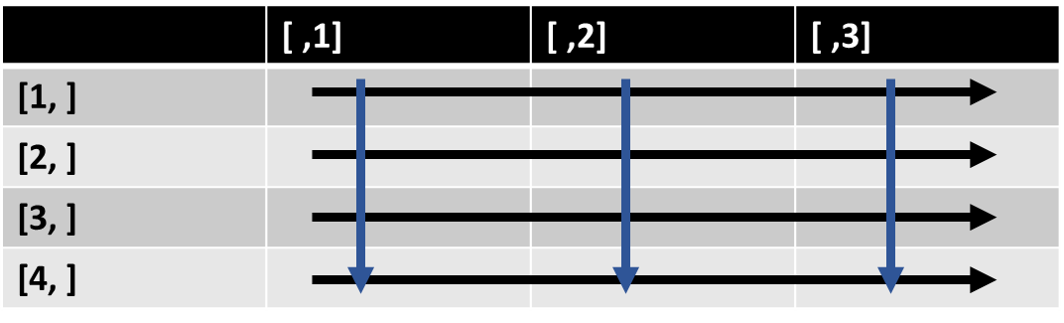
\includegraphics[width=0.8\linewidth]{figs/matrix} 

}

\caption{R matrix, each row and each column are vectors}\label{fig:unnamed-chunk-11}
\end{figure}

We can also use the class and is.x function to inspect the column and the matrix as a whole and see that it is indeed
both a vector and made of vectors.

\begin{Shaded}
\begin{Highlighting}[]
\FunctionTok{class}\NormalTok{(mat)}
\end{Highlighting}
\end{Shaded}

\begin{verbatim}
## [1] "matrix" "array"
\end{verbatim}

\begin{Shaded}
\begin{Highlighting}[]
\FunctionTok{class}\NormalTok{(mat[}\DecValTok{1}\NormalTok{,])}
\end{Highlighting}
\end{Shaded}

\begin{verbatim}
## [1] "numeric"
\end{verbatim}

\begin{Shaded}
\begin{Highlighting}[]
\FunctionTok{class}\NormalTok{(mat[,}\DecValTok{1}\NormalTok{])}
\end{Highlighting}
\end{Shaded}

\begin{verbatim}
## [1] "numeric"
\end{verbatim}

\begin{Shaded}
\begin{Highlighting}[]
\FunctionTok{is.numeric}\NormalTok{(mat)}
\end{Highlighting}
\end{Shaded}

\begin{verbatim}
## [1] TRUE
\end{verbatim}

\begin{Shaded}
\begin{Highlighting}[]
\FunctionTok{is.atomic}\NormalTok{(mat)}
\end{Highlighting}
\end{Shaded}

\begin{verbatim}
## [1] TRUE
\end{verbatim}

\begin{Shaded}
\begin{Highlighting}[]
\FunctionTok{is.atomic}\NormalTok{(mat[}\DecValTok{1}\NormalTok{,])}
\end{Highlighting}
\end{Shaded}

\begin{verbatim}
## [1] TRUE
\end{verbatim}

\begin{center}\rule{0.5\linewidth}{0.5pt}\end{center}

\textbf{Quick R exercise}

There are several R functions that can be used to generate a matrix.

\begin{enumerate}
\def\labelenumi{\arabic{enumi}.}
\item
  Create a numeric vector of 10 elements, use the matrix function to convert is to a matrix with 5 rows and two columns, what happens when the argument byrow is set to TRUE?
\item
  Create a character vector of 10 element use the function cbind to bind it with the vector from the previous question. Are the vectors columns or rows? What happens when you use the function rbind?
\item
  Use the typeof function on one of the matrices from question 2, what type of data does this matrix contain, what does it tell you about the coercion of data type within a matrix?
\end{enumerate}

\begin{center}\rule{0.5\linewidth}{0.5pt}\end{center}

\hypertarget{working-with-matrices}{%
\subsection{\texorpdfstring{\textbf{Working with matrices}}{Working with matrices}}\label{working-with-matrices}}

A matrix is basically a vector with two dimensions when a matrix is indexed like a vector, i.e.
matrix{[}n{]}. By default, when a matrix is indexed in that manor R will return the value found on the
nth position of the original vector (see snippet bellow).
One of R strength is that it allows to also index and access any combination of columns and rows,
not just individual elements. This is done similar to accessing a vector only the positions of the
rows and columns are separated by a comma, e.g.~matrix{[}row,column{]}. This form of indexing allows to
subset specific rows and columns from the matrix, as demonstrated in the snippet bellow.

\begin{Shaded}
\begin{Highlighting}[]
\CommentTok{\#Mat[5] will output the element occupaing the fifth position of the vector used to construct the}
\CommentTok{\#matrix i.e. 3.9}
\NormalTok{mat[}\DecValTok{5}\NormalTok{]}
\end{Highlighting}
\end{Shaded}

\begin{verbatim}
## [1] 3.9
\end{verbatim}

\begin{Shaded}
\begin{Highlighting}[]
\CommentTok{\#Mat[,1] will output the first column of the matrix}
\NormalTok{mat[,}\DecValTok{1}\NormalTok{]}
\end{Highlighting}
\end{Shaded}

\begin{verbatim}
## [1] 3.5 3.6 3.7 3.8
\end{verbatim}

\begin{Shaded}
\begin{Highlighting}[]
\CommentTok{\#mat[,2:3] will output the 2nd and 3rd columns of the matrix }

\NormalTok{mat[,}\DecValTok{2}\SpecialCharTok{:}\DecValTok{3}\NormalTok{]}
\end{Highlighting}
\end{Shaded}

\begin{verbatim}
##      [,1] [,2]
## [1,]  3.9  4.3
## [2,]  4.0  4.4
## [3,]  4.1  4.5
## [4,]  4.2  4.6
\end{verbatim}

\begin{Shaded}
\begin{Highlighting}[]
\CommentTok{\#mat[1,] will output the first row of the matrix}
\NormalTok{mat[}\DecValTok{1}\NormalTok{,]}
\end{Highlighting}
\end{Shaded}

\begin{verbatim}
## [1] 3.5 3.9 4.3
\end{verbatim}

\begin{Shaded}
\begin{Highlighting}[]
\CommentTok{\#mat[1:2,] will output the first 2 rows of the matrix}
\NormalTok{mat[}\DecValTok{1}\SpecialCharTok{:}\DecValTok{2}\NormalTok{,]}
\end{Highlighting}
\end{Shaded}

\begin{verbatim}
##      [,1] [,2] [,3]
## [1,]  3.5  3.9  4.3
## [2,]  3.6  4.0  4.4
\end{verbatim}

\begin{Shaded}
\begin{Highlighting}[]
\CommentTok{\#mat[1:2,1:2] will subset the first two rows and columns of the matrix}
\NormalTok{mat[}\DecValTok{1}\SpecialCharTok{:}\DecValTok{2}\NormalTok{,}\DecValTok{1}\SpecialCharTok{:}\DecValTok{2}\NormalTok{]}
\end{Highlighting}
\end{Shaded}

\begin{verbatim}
##      [,1] [,2]
## [1,]  3.5  3.9
## [2,]  3.6  4.0
\end{verbatim}

\begin{Shaded}
\begin{Highlighting}[]
\CommentTok{\#The rows and colums of a matrix can be named, so that the vactors have meaningfull names.}
\CommentTok{\#This is done using the function colnames and rownames}

\NormalTok{stud\_mrks }\OtherTok{\textless{}{-}}\NormalTok{ mat}
\NormalTok{rn }\OtherTok{\textless{}{-}} \FunctionTok{c}\NormalTok{(}\StringTok{"Class1"}\NormalTok{,}\StringTok{"Class2"}\NormalTok{,}\StringTok{"Class3"}\NormalTok{,}\StringTok{"Class4"}\NormalTok{)}
\NormalTok{cn }\OtherTok{\textless{}{-}} \FunctionTok{c}\NormalTok{(}\StringTok{"Student1"}\NormalTok{,}\StringTok{"Student2"}\NormalTok{,}\StringTok{"Student3"}\NormalTok{)}
\FunctionTok{rownames}\NormalTok{(stud\_mrks) }\OtherTok{\textless{}{-}}\NormalTok{ rn}
\FunctionTok{colnames}\NormalTok{(stud\_mrks) }\OtherTok{\textless{}{-}}\NormalTok{ cn}

\NormalTok{stud\_mrks}
\end{Highlighting}
\end{Shaded}

\begin{verbatim}
##        Student1 Student2 Student3
## Class1      3.5      3.9      4.3
## Class2      3.6      4.0      4.4
## Class3      3.7      4.1      4.5
## Class4      3.8      4.2      4.6
\end{verbatim}

\begin{Shaded}
\begin{Highlighting}[]
\CommentTok{\#The names can be used to index the matrix, note the use of comma.}
\NormalTok{stud\_mrks[}\StringTok{"Class1"}\NormalTok{,]}
\end{Highlighting}
\end{Shaded}

\begin{verbatim}
## Student1 Student2 Student3 
##      3.5      3.9      4.3
\end{verbatim}

\begin{Shaded}
\begin{Highlighting}[]
\NormalTok{stud\_mrks[,}\StringTok{"Student1"}\NormalTok{]}
\end{Highlighting}
\end{Shaded}

\begin{verbatim}
## Class1 Class2 Class3 Class4 
##    3.5    3.6    3.7    3.8
\end{verbatim}

\begin{center}\rule{0.5\linewidth}{0.5pt}\end{center}

\textbf{Quick R exercise}

\begin{enumerate}
\def\labelenumi{\arabic{enumi}.}
\item
  Assign the matrix mat to the variable mat\_bs and replace the first row of mat\_bs with A,B,C
\item
  Replace the 4th element in the matrix mat\_bs with 1000
\item
  Assign the 3rd column of the matrix mat\_bs the the vector v\_bs
\item
  Use the function t to transform the matrix mat\_bs, how many rows does it have now?
\end{enumerate}

\begin{center}\rule{0.5\linewidth}{0.5pt}\end{center}

One of R's greatest strength is the ability to perform tasks on a matrix as a whole, negating the need to use a loop
every time an operation is needed to be done on several columns.

\begin{Shaded}
\begin{Highlighting}[]
\CommentTok{\#Let\textquotesingle{}s generate a new matrix, this time with matrix function}
\CommentTok{\#byrow, fill the matrix by rows}
\NormalTok{mat2 }\OtherTok{\textless{}{-}} \FunctionTok{matrix}\NormalTok{(}\FunctionTok{sample}\NormalTok{(}\DecValTok{1}\SpecialCharTok{:}\DecValTok{1000}\NormalTok{,}\DecValTok{100}\NormalTok{,}\AttributeTok{replace=}\NormalTok{F),}\AttributeTok{nrow =} \DecValTok{10}\NormalTok{,}\AttributeTok{ncol =} \DecValTok{10}\NormalTok{,}\AttributeTok{byrow =}\NormalTok{ T)}
\FunctionTok{head}\NormalTok{(mat2)}
\end{Highlighting}
\end{Shaded}

\begin{verbatim}
##      [,1] [,2] [,3] [,4] [,5] [,6] [,7] [,8] [,9] [,10]
## [1,]  859  449  110  675  232  893  619  974  271   630
## [2,]  531  621  753  366  157  866  135  705   21   769
## [3,]  886  990   98  823  586  411  150  783  776   382
## [4,]  937  652  540  327  239  741  951   46  681   842
## [5,]  903  670  947  446  785  661   53  646   12   113
## [6,]   25  538  433  763  227  622   71  173  521   762
\end{verbatim}

\begin{Shaded}
\begin{Highlighting}[]
\CommentTok{\#When handling data, there is sometimes a need to transform it.}
\CommentTok{\#Log transformation is a common one. R\textquotesingle{}s handling of matrices allows to do it without resorting to a for loop.}
\CommentTok{\#Note that I am copying the matrix because I still want to use the original}
\NormalTok{mat2\_log }\OtherTok{\textless{}{-}} \FunctionTok{log10}\NormalTok{(mat2)}
\FunctionTok{head}\NormalTok{(mat2\_log)}
\end{Highlighting}
\end{Shaded}

\begin{verbatim}
##          [,1]     [,2]     [,3]     [,4]     [,5]     [,6]     [,7]     [,8]
## [1,] 2.933993 2.652246 2.041393 2.829304 2.365488 2.950851 2.791691 2.988559
## [2,] 2.725095 2.793092 2.876795 2.563481 2.195900 2.937518 2.130334 2.848189
## [3,] 2.947434 2.995635 1.991226 2.915400 2.767898 2.613842 2.176091 2.893762
## [4,] 2.971740 2.814248 2.732394 2.514548 2.378398 2.869818 2.978181 1.662758
## [5,] 2.955688 2.826075 2.976350 2.649335 2.894870 2.820201 1.724276 2.810233
## [6,] 1.397940 2.730782 2.636488 2.882525 2.356026 2.793790 1.851258 2.238046
##          [,9]    [,10]
## [1,] 2.432969 2.799341
## [2,] 1.322219 2.885926
## [3,] 2.889862 2.582063
## [4,] 2.833147 2.925312
## [5,] 1.079181 2.053078
## [6,] 2.716838 2.881955
\end{verbatim}

\begin{Shaded}
\begin{Highlighting}[]
\CommentTok{\#Another common transformation is to calculate the proportion of value in the column or raw (often referred to as normalizing the data). R makes it easy to normalize matrices by rows or columns.}
\CommentTok{\#All that\textquotesingle{}s needed to do is to divide the matrix by the sum of its columns or rows}

\NormalTok{mat2\_freq\_row }\OtherTok{\textless{}{-}}\NormalTok{ mat2}\SpecialCharTok{/}\FunctionTok{rowSums}\NormalTok{(mat2)}
\FunctionTok{head}\NormalTok{(mat2\_freq\_row)}
\end{Highlighting}
\end{Shaded}

\begin{verbatim}
##             [,1]       [,2]       [,3]       [,4]       [,5]       [,6]
## [1,] 0.150385154 0.07860644 0.01925770 0.11817227 0.04061625 0.15633754
## [2,] 0.107839155 0.12611698 0.15292445 0.07432981 0.03188465 0.17587327
## [3,] 0.150552251 0.16822430 0.01665251 0.13984707 0.09957519 0.06983857
## [4,] 0.157320349 0.10946944 0.09066488 0.05490262 0.04012760 0.12441236
## [5,] 0.172459893 0.12796028 0.18086325 0.08517953 0.14992361 0.12624141
## [6,] 0.006045949 0.13010883 0.10471584 0.18452237 0.05489722 0.15042322
##            [,7]        [,8]        [,9]      [,10]
## [1,] 0.10836835 0.170518207 0.047443978 0.11029412
## [2,] 0.02741673 0.143176279 0.004264825 0.15617384
## [3,] 0.02548853 0.133050127 0.131860663 0.06491079
## [4,] 0.15967092 0.007723304 0.114338482 0.14137005
## [5,] 0.01012223 0.123376623 0.002291826 0.02158136
## [6,] 0.01717050 0.041837969 0.125997582 0.18428053
\end{verbatim}

\begin{Shaded}
\begin{Highlighting}[]
\CommentTok{\#rowSums should be 1}
\FunctionTok{rowSums}\NormalTok{(mat2\_freq\_row)}
\end{Highlighting}
\end{Shaded}

\begin{verbatim}
##  [1] 1 1 1 1 1 1 1 1 1 1
\end{verbatim}

\begin{Shaded}
\begin{Highlighting}[]
\CommentTok{\#When normalizing by column it is impossible to just use the "/" operator, due to the way R stores matrices. Need to use the sweep function. This is not an issue when normalizing by rows.}
\CommentTok{\#use ?sweep to see which each of the arguments means.}

\NormalTok{mat2\_freq\_columns }\OtherTok{\textless{}{-}} \FunctionTok{sweep}\NormalTok{(mat2,}\DecValTok{2}\NormalTok{,}\FunctionTok{colSums}\NormalTok{(mat2),}\StringTok{"/"}\NormalTok{)}
\FunctionTok{head}\NormalTok{(mat2\_freq\_columns)}
\end{Highlighting}
\end{Shaded}

\begin{verbatim}
##             [,1]       [,2]       [,3]       [,4]       [,5]       [,6]
## [1,] 0.141492341 0.07405575 0.01941405 0.12525515 0.04458109 0.11777895
## [2,] 0.087464998 0.10242454 0.13289799 0.06791613 0.03016910 0.11421788
## [3,] 0.145939713 0.16328550 0.01729615 0.15271850 0.11260569 0.05420733
## [4,] 0.154340306 0.10753752 0.09530533 0.06067916 0.04592621 0.09773147
## [5,] 0.148739911 0.11050635 0.16713731 0.08276118 0.15084550 0.08718016
## [6,] 0.004117938 0.08873495 0.07642076 0.14158471 0.04362029 0.08203640
##            [,7]        [,8]        [,9]      [,10]
## [1,] 0.16027965 0.204407135 0.057684121 0.10607846
## [2,] 0.03495598 0.147953830 0.004469987 0.12948308
## [3,] 0.03883998 0.164323190 0.165176671 0.06432059
## [4,] 0.24624547 0.009653725 0.144955300 0.14177471
## [5,] 0.01372346 0.135571878 0.002554278 0.01902677
## [6,] 0.01838426 0.036306401 0.110898255 0.12830443
\end{verbatim}

\begin{Shaded}
\begin{Highlighting}[]
\CommentTok{\#If everything worked out the sum of each column should be 1 now}
\FunctionTok{colSums}\NormalTok{(mat2\_freq\_columns)}
\end{Highlighting}
\end{Shaded}

\begin{verbatim}
##  [1] 1 1 1 1 1 1 1 1 1 1
\end{verbatim}

\begin{Shaded}
\begin{Highlighting}[]
\CommentTok{\#Just like vectors it is also possible to preform mathematical operations on two matrices}
\NormalTok{mat2\_mlt }\OtherTok{\textless{}{-}}\NormalTok{ mat2\_freq\_columns}\SpecialCharTok{*}\NormalTok{mat2\_log}
\FunctionTok{head}\NormalTok{(mat2\_mlt)}
\end{Highlighting}
\end{Shaded}

\begin{verbatim}
##            [,1]      [,2]       [,3]      [,4]       [,5]      [,6]       [,7]
## [1,] 0.41513756 0.1964141 0.03963170 0.3543849 0.10545604 0.3475482 0.44745119
## [2,] 0.23835039 0.2860811 0.38232026 0.1741017 0.06624832 0.3355171 0.07446791
## [3,] 0.43014763 0.4891438 0.03444055 0.4452355 0.31168102 0.1416894 0.08451934
## [4,] 0.45865920 0.3026372 0.26041169 0.1525806 0.10923080 0.2804716 0.73336346
## [5,] 0.43962873 0.3122992 0.49745913 0.2192621 0.43667807 0.2458656 0.02366303
## [6,] 0.00575663 0.2423158 0.20148240 0.4081214 0.10277054 0.2291925 0.03403401
##            [,8]        [,9]      [,10]
## [1,] 0.61088278 0.140343695 0.29694975
## [2,] 0.42140049 0.005910303 0.37367863
## [3,] 0.47551216 0.477337739 0.16607985
## [4,] 0.01605181 0.410679690 0.41473527
## [5,] 0.38098850 0.002756529 0.03906346
## [6,] 0.08125540 0.301292561 0.36976759
\end{verbatim}

Because matrices are tables but behave like vectors, operating on them is memory efficient and many R packages use
them as a preferred object.

\hypertarget{lists}{%
\section{\texorpdfstring{\textbf{Lists}}{Lists}}\label{lists}}

A list is a multidimensional vector, which is a fancy way of saying that a list is a vector that can house any R
object as an element.
The elements of a list are independent of each other, making it a great object to store the output of function that
handle data. For example some functions from the stringer package output their result as lists. Especially those with
\_all suffix.

The code snippet bellow demonstrate how to create lists, as always there is more than one way to obtain your goal.

\begin{Shaded}
\begin{Highlighting}[]
\CommentTok{\#creating an empty list of 10 elements}
\CommentTok{\#Because a list is basically a vector of elements, it is possible to creat it using the vector function}
\NormalTok{list1 }\OtherTok{\textless{}{-}} \FunctionTok{vector}\NormalTok{(}\AttributeTok{mode =} \StringTok{"list"}\NormalTok{, }\AttributeTok{length =} \DecValTok{10}\NormalTok{)}
\FunctionTok{class}\NormalTok{(list1)}
\end{Highlighting}
\end{Shaded}

\begin{verbatim}
## [1] "list"
\end{verbatim}

\begin{Shaded}
\begin{Highlighting}[]
\FunctionTok{is.vector}\NormalTok{(list1)}
\end{Highlighting}
\end{Shaded}

\begin{verbatim}
## [1] TRUE
\end{verbatim}

\begin{Shaded}
\begin{Highlighting}[]
\FunctionTok{is.atomic}\NormalTok{(list1) }\CommentTok{\#why is it not atomic?}
\end{Highlighting}
\end{Shaded}

\begin{verbatim}
## [1] FALSE
\end{verbatim}

\begin{Shaded}
\begin{Highlighting}[]
\FunctionTok{head}\NormalTok{(list1,}\DecValTok{3}\NormalTok{)}
\end{Highlighting}
\end{Shaded}

\begin{verbatim}
## [[1]]
## NULL
## 
## [[2]]
## NULL
## 
## [[3]]
## NULL
\end{verbatim}

\begin{Shaded}
\begin{Highlighting}[]
\CommentTok{\#Creating a list by using the list function}
\NormalTok{list2 }\OtherTok{\textless{}{-}} \FunctionTok{list}\NormalTok{(}\FunctionTok{matrix}\NormalTok{(}\FunctionTok{sample}\NormalTok{(}\DecValTok{10}\SpecialCharTok{:}\DecValTok{1000}\NormalTok{,}\DecValTok{100}\NormalTok{,}\AttributeTok{replace =}\NormalTok{ F),}\AttributeTok{ncol =} \DecValTok{2}\NormalTok{),}
                    \FunctionTok{cbind}\NormalTok{(}\FunctionTok{seq}\NormalTok{(}\DecValTok{1}\NormalTok{,}\DecValTok{100}\NormalTok{,}\AttributeTok{by=}\DecValTok{2}\NormalTok{),}\FunctionTok{rep}\NormalTok{(}\DecValTok{10}\NormalTok{,}\DecValTok{50}\NormalTok{)),}\FunctionTok{c}\NormalTok{(}\StringTok{"Category1"}\NormalTok{,}\StringTok{"Category2"}\NormalTok{),list1,}
              \FunctionTok{factor}\NormalTok{(}\FunctionTok{c}\NormalTok{(}\StringTok{"Cat"}\NormalTok{,}\StringTok{"Dog"}\NormalTok{,}\StringTok{"Cat"}\NormalTok{,}\StringTok{"Mouse"}\NormalTok{)) )}
\end{Highlighting}
\end{Shaded}

\hypertarget{working-with-lists}{%
\subsection{\texorpdfstring{\textbf{Working with lists}}{Working with lists}}\label{working-with-lists}}

The previous snippet demonstrated that lists can store any type of R object, even other lists.
As mentioned, the elements of a list are independent of each other and in order to modify them they need to be
accessed individually.
Since lists are vectors, each element can be inspected, like one would inspect a vector.

\begin{Shaded}
\begin{Highlighting}[]
\CommentTok{\#Inspecting the 3rd element of list2}
\NormalTok{list2[}\DecValTok{3}\NormalTok{]}
\end{Highlighting}
\end{Shaded}

\begin{verbatim}
## [[1]]
## [1] "Category1" "Category2"
\end{verbatim}

However, indexing a list like a vector does not allow you to modify the element

\begin{Shaded}
\begin{Highlighting}[]
\CommentTok{\#Note how the head function is unable to truncate the element to its first 2 componenets}
\FunctionTok{head}\NormalTok{(list2[}\DecValTok{5}\NormalTok{],}\DecValTok{2}\NormalTok{)}
\end{Highlighting}
\end{Shaded}

\begin{verbatim}
## [[1]]
## [1] Cat   Dog   Cat   Mouse
## Levels: Cat Dog Mouse
\end{verbatim}

\begin{Shaded}
\begin{Highlighting}[]
\CommentTok{\#Note how indexing like a vector does not allow you to subset the element itself}
\NormalTok{list2[}\DecValTok{5}\NormalTok{][}\DecValTok{1}\NormalTok{]}
\end{Highlighting}
\end{Shaded}

\begin{verbatim}
## [[1]]
## [1] Cat   Dog   Cat   Mouse
## Levels: Cat Dog Mouse
\end{verbatim}

In case you noticed, when using the head function on a list each element is sounded by double square brackets ( {[}{[} ).
When subseting a list with {[}, it will always return another list. Think of it elements one on a character vector
where each element is a string. You can see each string even replace them but can't modify them. In order to access
and modify an element of the list {[}{[} have to be used.

\begin{Shaded}
\begin{Highlighting}[]
\CommentTok{\#Subseting the last element of list2 and assigning it to the first element of list1}
\NormalTok{list1[[}\DecValTok{1}\NormalTok{]] }\OtherTok{\textless{}{-}}\NormalTok{ list2[[}\DecValTok{5}\NormalTok{]][}\DecValTok{1}\SpecialCharTok{:}\DecValTok{3}\NormalTok{]}
\NormalTok{list1[}\DecValTok{1}\NormalTok{]}
\end{Highlighting}
\end{Shaded}

\begin{verbatim}
## [[1]]
## [1] Cat Dog Cat
## Levels: Cat Dog Mouse
\end{verbatim}

\hypertarget{lists-and-the-operator}{%
\subsection{\texorpdfstring{\textbf{Lists and the \$ operator}}{Lists and the \$ operator}}\label{lists-and-the-operator}}

\$ is an operator that can be thought of as the equivalent of {[}{[} {]}{]}, therefore it can be used to access elements of a list. However, in order to use it the elements must be named first.

\begin{Shaded}
\begin{Highlighting}[]
\CommentTok{\#Are the elements of list2 named?}
\FunctionTok{names}\NormalTok{(list2)}
\end{Highlighting}
\end{Shaded}

\begin{verbatim}
## NULL
\end{verbatim}

\begin{Shaded}
\begin{Highlighting}[]
\CommentTok{\#Naming the elements of the list}
\FunctionTok{names}\NormalTok{(list2) }\OtherTok{\textless{}{-}} \FunctionTok{c}\NormalTok{(}\StringTok{"Sample1"}\NormalTok{,}\StringTok{"Sample2"}\NormalTok{,}\StringTok{"Categories"}\NormalTok{,}\StringTok{"Nested\_list"}\NormalTok{,}\StringTok{"Pets"}\NormalTok{)}

\FunctionTok{names}\NormalTok{(list2)}
\end{Highlighting}
\end{Shaded}

\begin{verbatim}
## [1] "Sample1"     "Sample2"     "Categories"  "Nested_list" "Pets"
\end{verbatim}

\begin{Shaded}
\begin{Highlighting}[]
\CommentTok{\#Accessing the list using $, note how rstudio autocompletes the elements}
\NormalTok{list2}\SpecialCharTok{$}\NormalTok{Categories}
\end{Highlighting}
\end{Shaded}

\begin{verbatim}
## [1] "Category1" "Category2"
\end{verbatim}

\begin{Shaded}
\begin{Highlighting}[]
\NormalTok{list2}\SpecialCharTok{$}\NormalTok{Categories[}\DecValTok{2}\NormalTok{]}
\end{Highlighting}
\end{Shaded}

\begin{verbatim}
## [1] "Category2"
\end{verbatim}

\begin{Shaded}
\begin{Highlighting}[]
\NormalTok{list2}\SpecialCharTok{$}\NormalTok{Sample2[}\DecValTok{1}\NormalTok{,}\DecValTok{2}\NormalTok{]}
\end{Highlighting}
\end{Shaded}

\begin{verbatim}
## [1] 10
\end{verbatim}

\begin{Shaded}
\begin{Highlighting}[]
\NormalTok{list2}\SpecialCharTok{$}\NormalTok{Sample2[}\DecValTok{1}\NormalTok{,}\DecValTok{2}\NormalTok{] }\OtherTok{\textless{}{-}} \DecValTok{11}
\NormalTok{list2}\SpecialCharTok{$}\NormalTok{Sample2[}\DecValTok{1}\NormalTok{,}\DecValTok{2}\NormalTok{]}
\end{Highlighting}
\end{Shaded}

\begin{verbatim}
## [1] 11
\end{verbatim}

\begin{center}\rule{0.5\linewidth}{0.5pt}\end{center}

\textbf{Quick R exercise}

Let's wrap up working with lists with the following exercise:

\begin{enumerate}
\def\labelenumi{\arabic{enumi}.}
\tightlist
\item
  Change the values of the 10th raw in sample2 to 7 and 5
\item
  Log10 transform Sample2 and assign it to the first element of list1
\item
  Name the first element of list1 ``S2\_log''
\item
  Use sweep to normalize Sample1 by dividing it by the sum of its columns, assign it to the 2nd element of list1 and name is S1\_norm
\item
  Create a list called list3 that contains only the first 2 elements of list1
\end{enumerate}

\begin{center}\rule{0.5\linewidth}{0.5pt}\end{center}

\hypertarget{data.frames}{%
\section{\texorpdfstring{\textbf{data.frames}}{data.frames}}\label{data.frames}}

Data frames are a commonly used objects in R especially in data preparation and analysis.
Data frames are a special case of a list containing vectors of equal length as element, giving it a rectangular shape. The vectors make up the columns of the dataframe.

Let's create a datafram or two

\begin{Shaded}
\begin{Highlighting}[]
\CommentTok{\# datafeames can be created by using the data.frame function}
\CommentTok{\#Note that by default strings are coereced to factors, which can be annoying}
\NormalTok{df1 }\OtherTok{\textless{}{-}} \FunctionTok{data.frame}\NormalTok{(}\AttributeTok{X =} \FunctionTok{seq}\NormalTok{(}\DecValTok{1}\NormalTok{,}\DecValTok{10}\NormalTok{, }\AttributeTok{by =} \DecValTok{1}\NormalTok{), }
                  \AttributeTok{Y =} \FunctionTok{seq}\NormalTok{(}\DecValTok{100}\NormalTok{,}\DecValTok{1000}\NormalTok{, }\AttributeTok{by =} \DecValTok{100}\NormalTok{),}
                  \AttributeTok{Z =}\NormalTok{ LETTERS[}\DecValTok{1}\SpecialCharTok{:}\DecValTok{10}\NormalTok{], }\AttributeTok{stringsAsFactors =}\NormalTok{ F)}

\CommentTok{\#Each column is an independent vector, that\textquotesingle{}s why columns X and Y can be numeric and Z a character.}
\FunctionTok{str}\NormalTok{(df1)}
\end{Highlighting}
\end{Shaded}

\begin{verbatim}
## 'data.frame':    10 obs. of  3 variables:
##  $ X: num  1 2 3 4 5 6 7 8 9 10
##  $ Y: num  100 200 300 400 500 600 700 800 900 1000
##  $ Z: chr  "A" "B" "C" "D" ...
\end{verbatim}

\begin{Shaded}
\begin{Highlighting}[]
\CommentTok{\# It is also possible to coerce a matrix to a dataframe}

\NormalTok{df2 }\OtherTok{\textless{}{-}} \FunctionTok{as.data.frame}\NormalTok{(mat2)}

\CommentTok{\#let\textquotesingle{}s see what a dataframe looks like}
\FunctionTok{head}\NormalTok{(df1,}\DecValTok{4}\NormalTok{)}
\end{Highlighting}
\end{Shaded}

\begin{verbatim}
##   X   Y Z
## 1 1 100 A
## 2 2 200 B
## 3 3 300 C
## 4 4 400 D
\end{verbatim}

\begin{Shaded}
\begin{Highlighting}[]
\FunctionTok{head}\NormalTok{(df2,}\DecValTok{4}\NormalTok{)}
\end{Highlighting}
\end{Shaded}

\begin{verbatim}
##    V1  V2  V3  V4  V5  V6  V7  V8  V9 V10
## 1 859 449 110 675 232 893 619 974 271 630
## 2 531 621 753 366 157 866 135 705  21 769
## 3 886 990  98 823 586 411 150 783 776 382
## 4 937 652 540 327 239 741 951  46 681 842
\end{verbatim}

As can be seen in the output of the head function all the columns of the dataframes are named.
This is an attribute of dataframes. The name of the columns can be accessed and changed with the function colnames. The nameless column to the left is not a real column, it is the name of each row. This can be accessed by the function rownames.

\begin{Shaded}
\begin{Highlighting}[]
\FunctionTok{colnames}\NormalTok{(df1)}
\end{Highlighting}
\end{Shaded}

\begin{verbatim}
## [1] "X" "Y" "Z"
\end{verbatim}

\begin{Shaded}
\begin{Highlighting}[]
\FunctionTok{colnames}\NormalTok{(df1)[}\DecValTok{1}\NormalTok{] }\OtherTok{\textless{}{-}} \StringTok{"Sample1"}
\FunctionTok{colnames}\NormalTok{(df1)}
\end{Highlighting}
\end{Shaded}

\begin{verbatim}
## [1] "Sample1" "Y"       "Z"
\end{verbatim}

\begin{Shaded}
\begin{Highlighting}[]
\FunctionTok{head}\NormalTok{(}\FunctionTok{rownames}\NormalTok{(df2),}\DecValTok{3}\NormalTok{)}
\end{Highlighting}
\end{Shaded}

\begin{verbatim}
## [1] "1" "2" "3"
\end{verbatim}

\begin{Shaded}
\begin{Highlighting}[]
\FunctionTok{rownames}\NormalTok{(df2) }\OtherTok{\textless{}{-}}\NormalTok{ LETTERS[}\DecValTok{1}\SpecialCharTok{:}\FunctionTok{nrow}\NormalTok{(df2)]}
\FunctionTok{head}\NormalTok{(}\FunctionTok{rownames}\NormalTok{(df2),}\DecValTok{3}\NormalTok{)}
\end{Highlighting}
\end{Shaded}

\begin{verbatim}
## [1] "A" "B" "C"
\end{verbatim}

Dataframes behave both like a list and like matrix. Because the columns are named, they can be accessed by the \$ operator. However just like matrices they can also be subset by {[}. Just like matrices, operations on dataframes can be vectorized.

Let's look at some examples of how to work with dataframes

\begin{Shaded}
\begin{Highlighting}[]
\CommentTok{\#accesing a single column using the $ operator}
\NormalTok{df1}\SpecialCharTok{$}\NormalTok{Sample1}
\end{Highlighting}
\end{Shaded}

\begin{verbatim}
##  [1]  1  2  3  4  5  6  7  8  9 10
\end{verbatim}

\begin{Shaded}
\begin{Highlighting}[]
\CommentTok{\#subseting a dataframe using []}
\CommentTok{\#If no commas are used this is like subseting a list }
\NormalTok{df1[}\DecValTok{1}\SpecialCharTok{:}\DecValTok{2}\NormalTok{]}
\end{Highlighting}
\end{Shaded}

\begin{verbatim}
##    Sample1    Y
## 1        1  100
## 2        2  200
## 3        3  300
## 4        4  400
## 5        5  500
## 6        6  600
## 7        7  700
## 8        8  800
## 9        9  900
## 10      10 1000
\end{verbatim}

\begin{Shaded}
\begin{Highlighting}[]
\CommentTok{\#Like a matrix (i.e. 2D)}
\NormalTok{df1[,}\DecValTok{1}\NormalTok{]}
\end{Highlighting}
\end{Shaded}

\begin{verbatim}
##  [1]  1  2  3  4  5  6  7  8  9 10
\end{verbatim}

\begin{Shaded}
\begin{Highlighting}[]
\CommentTok{\#First 3 rows, and first 2 columns}
\NormalTok{df1[}\DecValTok{1}\SpecialCharTok{:}\DecValTok{3}\NormalTok{,}\DecValTok{1}\SpecialCharTok{:}\DecValTok{2}\NormalTok{]}
\end{Highlighting}
\end{Shaded}

\begin{verbatim}
##   Sample1   Y
## 1       1 100
## 2       2 200
## 3       3 300
\end{verbatim}

\begin{Shaded}
\begin{Highlighting}[]
\CommentTok{\#Adding a column to the dataframe}
\NormalTok{df1}\SpecialCharTok{$}\NormalTok{New\_column }\OtherTok{\textless{}{-}}\NormalTok{ df2}\SpecialCharTok{$}\NormalTok{V1}

\CommentTok{\#adding a new row to a dataframe}
\NormalTok{df1[}\FunctionTok{nrow}\NormalTok{(df1)}\SpecialCharTok{+}\DecValTok{1}\NormalTok{,] }\OtherTok{\textless{}{-}} \FunctionTok{c}\NormalTok{(}\DecValTok{1}\NormalTok{,}\DecValTok{1}\NormalTok{,}\DecValTok{1}\NormalTok{,}\DecValTok{1}\NormalTok{)}
\NormalTok{df1[}\FunctionTok{nrow}\NormalTok{(df1),]}
\end{Highlighting}
\end{Shaded}

\begin{verbatim}
##    Sample1 Y Z New_column
## 11       1 1 1          1
\end{verbatim}

\begin{Shaded}
\begin{Highlighting}[]
\CommentTok{\#Natural log transformation of a dataframe}
\NormalTok{df3 }\OtherTok{\textless{}{-}} \FunctionTok{log}\NormalTok{(df2)}
\FunctionTok{head}\NormalTok{(df3,}\DecValTok{3}\NormalTok{)}
\end{Highlighting}
\end{Shaded}

\begin{verbatim}
##         V1       V2       V3       V4       V5       V6       V7       V8
## A 6.755769 6.107023 4.700480 6.514713 5.446737 6.794587 6.428105 6.881411
## B 6.274762 6.431331 6.624065 5.902633 5.056246 6.763885 4.905275 6.558198
## C 6.786717 6.897705 4.584967 6.712956 6.373320 6.018593 5.010635 6.663133
##         V9      V10
## A 5.602119 6.445720
## B 3.044522 6.645091
## C 6.654153 5.945421
\end{verbatim}

\begin{center}\rule{0.5\linewidth}{0.5pt}\end{center}

\hypertarget{summary-exercise-lab1}{%
\chapter{\texorpdfstring{\textbf{Summary exercise Lab1}}{Summary exercise Lab1}}\label{summary-exercise-lab1}}

Start a script file in RStudio name it 3315\_lab1\_yourinitials.R
You will submit this script and output file if applicable to D2l submission folder by Tue Sept 20 23:59.

\textbf{1.} Create a vector containing the string ``How much wood would a woodchuck chuck if a woodchuck could chuck wood? He would chuck, he would, as much as he could, and chuck as much wood
As a woodchuck would if a woodchuck could chuck wood''

\begin{itemize}
\item
  How many elements does this vector contain? Show your work.
\item
  Count how many times does the word ``Wood'' appear in the vector
\end{itemize}

\textbf{2.} Create 3 identical strings of 10000 randomly selected polynucleotides and assign them to three vectors (do not copy one string three times)

\begin{itemize}
\item
  Show that they are identical
\item
  What is the \%GC in the string?
\end{itemize}

\textbf{3.} Create an empty list of 4 element

\textbf{4.} Name the elements E1-E4

\textbf{5.} Create a matrix from 3 numerical vectors each with 10 elements, assign it to the first element of the list

\textbf{6.} log10 transform the first element of the list and assign it to the 2 element of the list

\textbf{7.} Convert the first element of the list to a datafram and assign it to the 3 element of the list

\textbf{8.} Assign the dataframe to the 4th element of the list and add a 4th column of 10 letters

\textbf{9.} log10 transform the numeric columns of the dataframe occupying the 4th element of the list

\begin{center}\rule{0.5\linewidth}{0.5pt}\end{center}

\hypertarget{cross}{%
\chapter{Cross-references}\label{cross}}

Cross-references make it easier for your readers to find and link to elements in your book.

\hypertarget{chapters-and-sub-chapters}{%
\section{Chapters and sub-chapters}\label{chapters-and-sub-chapters}}

There are two steps to cross-reference any heading:

\begin{enumerate}
\def\labelenumi{\arabic{enumi}.}
\tightlist
\item
  Label the heading: \texttt{\#\ Hello\ world\ \{\#nice-label\}}.

  \begin{itemize}
  \tightlist
  \item
    Leave the label off if you like the automated heading generated based on your heading title: for example, \texttt{\#\ Hello\ world} = \texttt{\#\ Hello\ world\ \{\#hello-world\}}.
  \item
    To label an un-numbered heading, use: \texttt{\#\ Hello\ world\ \{-\#nice-label\}} or \texttt{\{\#\ Hello\ world\ .unnumbered\}}.
  \end{itemize}
\item
  Next, reference the labeled heading anywhere in the text using \texttt{\textbackslash{}@ref(nice-label)}; for example, please see Chapter \ref{cross}.

  \begin{itemize}
  \tightlist
  \item
    If you prefer text as the link instead of a numbered reference use: \protect\hyperlink{cross}{any text you want can go here}.
  \end{itemize}
\end{enumerate}

\hypertarget{captioned-figures-and-tables}{%
\section{Captioned figures and tables}\label{captioned-figures-and-tables}}

Figures and tables \emph{with captions} can also be cross-referenced from elsewhere in your book using \texttt{\textbackslash{}@ref(fig:chunk-label)} and \texttt{\textbackslash{}@ref(tab:chunk-label)}, respectively.

See Figure \ref{fig:nice-fig}.

\begin{Shaded}
\begin{Highlighting}[]
\FunctionTok{par}\NormalTok{(}\AttributeTok{mar =} \FunctionTok{c}\NormalTok{(}\DecValTok{4}\NormalTok{, }\DecValTok{4}\NormalTok{, .}\DecValTok{1}\NormalTok{, .}\DecValTok{1}\NormalTok{))}
\FunctionTok{plot}\NormalTok{(pressure, }\AttributeTok{type =} \StringTok{\textquotesingle{}b\textquotesingle{}}\NormalTok{, }\AttributeTok{pch =} \DecValTok{19}\NormalTok{)}
\end{Highlighting}
\end{Shaded}

\begin{figure}

{\centering 
\includegraphics[width=0.8\linewidth]{_main_files/figure-latex/nice-fig-1} 

}

\caption{Here is a nice figure!}\label{fig:nice-fig}
\end{figure}

Don't miss Table \ref{tab:nice-tab}.

\begin{Shaded}
\begin{Highlighting}[]
\NormalTok{knitr}\SpecialCharTok{::}\FunctionTok{kable}\NormalTok{(}
  \FunctionTok{head}\NormalTok{(pressure, }\DecValTok{10}\NormalTok{), }\AttributeTok{caption =} \StringTok{\textquotesingle{}Here is a nice table!\textquotesingle{}}\NormalTok{,}
  \AttributeTok{booktabs =} \ConstantTok{TRUE}
\NormalTok{)}
\end{Highlighting}
\end{Shaded}

\begin{table}

\caption{\label{tab:nice-tab}Here is a nice table!}
\centering
\begin{tabular}[t]{rr}
\toprule
temperature & pressure\\
\midrule
0 & 0.0002\\
20 & 0.0012\\
40 & 0.0060\\
60 & 0.0300\\
80 & 0.0900\\
\addlinespace
100 & 0.2700\\
120 & 0.7500\\
140 & 1.8500\\
160 & 4.2000\\
180 & 8.8000\\
\bottomrule
\end{tabular}
\end{table}

\hypertarget{parts}{%
\chapter{Parts}\label{parts}}

You can add parts to organize one or more book chapters together. Parts can be inserted at the top of an .Rmd file, before the first-level chapter heading in that same file.

Add a numbered part: \texttt{\#\ (PART)\ Act\ one\ \{-\}} (followed by \texttt{\#\ A\ chapter})

Add an unnumbered part: \texttt{\#\ (PART\textbackslash{}*)\ Act\ one\ \{-\}} (followed by \texttt{\#\ A\ chapter})

Add an appendix as a special kind of un-numbered part: \texttt{\#\ (APPENDIX)\ Other\ stuff\ \{-\}} (followed by \texttt{\#\ A\ chapter}). Chapters in an appendix are prepended with letters instead of numbers.

\hypertarget{footnotes-and-citations}{%
\chapter{Footnotes and citations}\label{footnotes-and-citations}}

\hypertarget{footnotes}{%
\section{Footnotes}\label{footnotes}}

Footnotes are put inside the square brackets after a caret \texttt{\^{}{[}{]}}. Like this one \footnote{This is a footnote.}.

\hypertarget{citations}{%
\section{Citations}\label{citations}}

Reference items in your bibliography file(s) using \texttt{@key}.

For example, we are using the \textbf{bookdown} package \citep{R-bookdown} (check out the last code chunk in index.Rmd to see how this citation key was added) in this sample book, which was built on top of R Markdown and \textbf{knitr} \citep{xie2015} (this citation was added manually in an external file book.bib).
Note that the \texttt{.bib} files need to be listed in the index.Rmd with the YAML \texttt{bibliography} key.

The RStudio Visual Markdown Editor can also make it easier to insert citations: \url{https://rstudio.github.io/visual-markdown-editing/\#/citations}

\hypertarget{blocks}{%
\chapter{Blocks}\label{blocks}}

\hypertarget{equations}{%
\section{Equations}\label{equations}}

Here is an equation.

\begin{equation} 
  f\left(k\right) = \binom{n}{k} p^k\left(1-p\right)^{n-k}
  \label{eq:binom}
\end{equation}

You may refer to using \texttt{\textbackslash{}@ref(eq:binom)}, like see Equation \eqref{eq:binom}.

\hypertarget{theorems-and-proofs}{%
\section{Theorems and proofs}\label{theorems-and-proofs}}

Labeled theorems can be referenced in text using \texttt{\textbackslash{}@ref(thm:tri)}, for example, check out this smart theorem \ref{thm:tri}.

\begin{theorem}
\protect\hypertarget{thm:tri}{}\label{thm:tri}For a right triangle, if \(c\) denotes the \emph{length} of the hypotenuse
and \(a\) and \(b\) denote the lengths of the \textbf{other} two sides, we have
\[a^2 + b^2 = c^2\]
\end{theorem}

Read more here \url{https://bookdown.org/yihui/bookdown/markdown-extensions-by-bookdown.html}.

\hypertarget{callout-blocks}{%
\section{Callout blocks}\label{callout-blocks}}

The R Markdown Cookbook provides more help on how to use custom blocks to design your own callouts: \url{https://bookdown.org/yihui/rmarkdown-cookbook/custom-blocks.html}

\hypertarget{sharing-your-book}{%
\chapter{Sharing your book}\label{sharing-your-book}}

\hypertarget{publishing}{%
\section{Publishing}\label{publishing}}

HTML books can be published online, see: \url{https://bookdown.org/yihui/bookdown/publishing.html}

\hypertarget{pages}{%
\section{404 pages}\label{pages}}

By default, users will be directed to a 404 page if they try to access a webpage that cannot be found. If you'd like to customize your 404 page instead of using the default, you may add either a \texttt{\_404.Rmd} or \texttt{\_404.md} file to your project root and use code and/or Markdown syntax.

\hypertarget{metadata-for-sharing}{%
\section{Metadata for sharing}\label{metadata-for-sharing}}

Bookdown HTML books will provide HTML metadata for social sharing on platforms like Twitter, Facebook, and LinkedIn, using information you provide in the \texttt{index.Rmd} YAML. To setup, set the \texttt{url} for your book and the path to your \texttt{cover-image} file. Your book's \texttt{title} and \texttt{description} are also used.

This \texttt{gitbook} uses the same social sharing data across all chapters in your book- all links shared will look the same.

Specify your book's source repository on GitHub using the \texttt{edit} key under the configuration options in the \texttt{\_output.yml} file, which allows users to suggest an edit by linking to a chapter's source file.

Read more about the features of this output format here:

\url{https://pkgs.rstudio.com/bookdown/reference/gitbook.html}

Or use:

\begin{Shaded}
\begin{Highlighting}[]
\NormalTok{?bookdown}\SpecialCharTok{::}\NormalTok{gitbook}
\end{Highlighting}
\end{Shaded}


  \bibliography{book.bib,packages.bib}

\end{document}
